% Use only LaTeX2e, calling the article.cls class and 12-point type.

\documentclass[12pt]{article}

% Users of the {thebibliography} environment or BibTeX should use the
% scicite.sty package, downloadable from *Science* at
% http://www.sciencemag.org/authors/preparing-manuscripts-using-latex 
% This package should properly format in-text
% reference calls and reference-list numbers.

%\usepackage{scicite}

\usepackage[utf8]{inputenc}
\usepackage{times}
\usepackage{amsmath}
\usepackage{graphicx}
\usepackage{graphics}
\usepackage{xcolor}
\usepackage{bm}
\usepackage{nicefrac}
\usepackage{pdfpages}
\usepackage{hyperref}
\usepackage{subcaption}
\usepackage{nameref}
\usepackage{listings}
%\usepackage{cite}
\usepackage{pdfpages}
\usepackage{afterpage}
\usepackage{enumerate}

\lstset { %
    language=C++,
    backgroundcolor=\color{black!5}, % set backgroundcolor
    basicstyle=\footnotesize,% basic font setting
}

\newcommand\blankpage{%
    \null
    \thispagestyle{empty}%
    \addtocounter{page}{-1}%
    \newpage}

\definecolor{applegreen}{rgb}{0.55, 0.71, 0.0}
\definecolor{forestgreen(web)}{rgb}{0.13, 0.55, 0.13}
\definecolor{harvardcrimson}{rgb}{0.79, 0.0, 0.09}

% The preamble here sets up a lot of new/revised commands and
% environments.  It's annoying, but please do *not* try to strip these
% out into a separate .sty file (which could lead to the loss of some
% information when we convert the file to other formats).  Instead, keep
% them in the preamble of your main LaTeX source file.


% The following parameters seem to provide a reasonable page setup.

\topmargin 0.0cm
\oddsidemargin 0.2cm
\textwidth 16cm 
\textheight 21cm
\footskip 1.0cm


%The next command sets up an environment for the abstract to your paper.

\newenvironment{sciabstract}{%
\begin{quote} \bf}
{\end{quote}}



% Include your paper's title here

\title{Research Plan\\
\vspace{1.8pt}
\large{for a Doctoral Study in Physics at the D-PHYS of ETH Zurich}} 


% Place the author information here.  Please hand-code the contact
% information and notecalls; do *not* use \footnote commands.  Let the
% author contact information appear immediately below the author names
% as shown.  We would also prefer that you don't change the type-size
% settings shown here.

\author
{Laura Paulina Šinkūnaitė}
%{John Smith,$^{1\ast}$ Jane Doe,$^{1}$ Joe Scientist$^{2}$\\
%\\
%\normalsize{$^{1}$Department of Chemistry, University of Wherever,}\\
%\normalsize{An Unknown Address, Wherever, ST 00000, USA}\\
%\normalsize{$^{2}$Another Unknown Address, Palookaville, ST 99999, USA}\\
%\\
%\normalsize{$^\ast$To whom correspondence should be addressed; E-mail:  jsmith@wherever.edu.}
%}

% Include the date command, but leave its argument blank.

\date{}



%%%%%%%%%%%%%%%%% END OF PREAMBLE %%%%%%%%%%%%%%%%


\begin{document} 

\begin{titlepage}
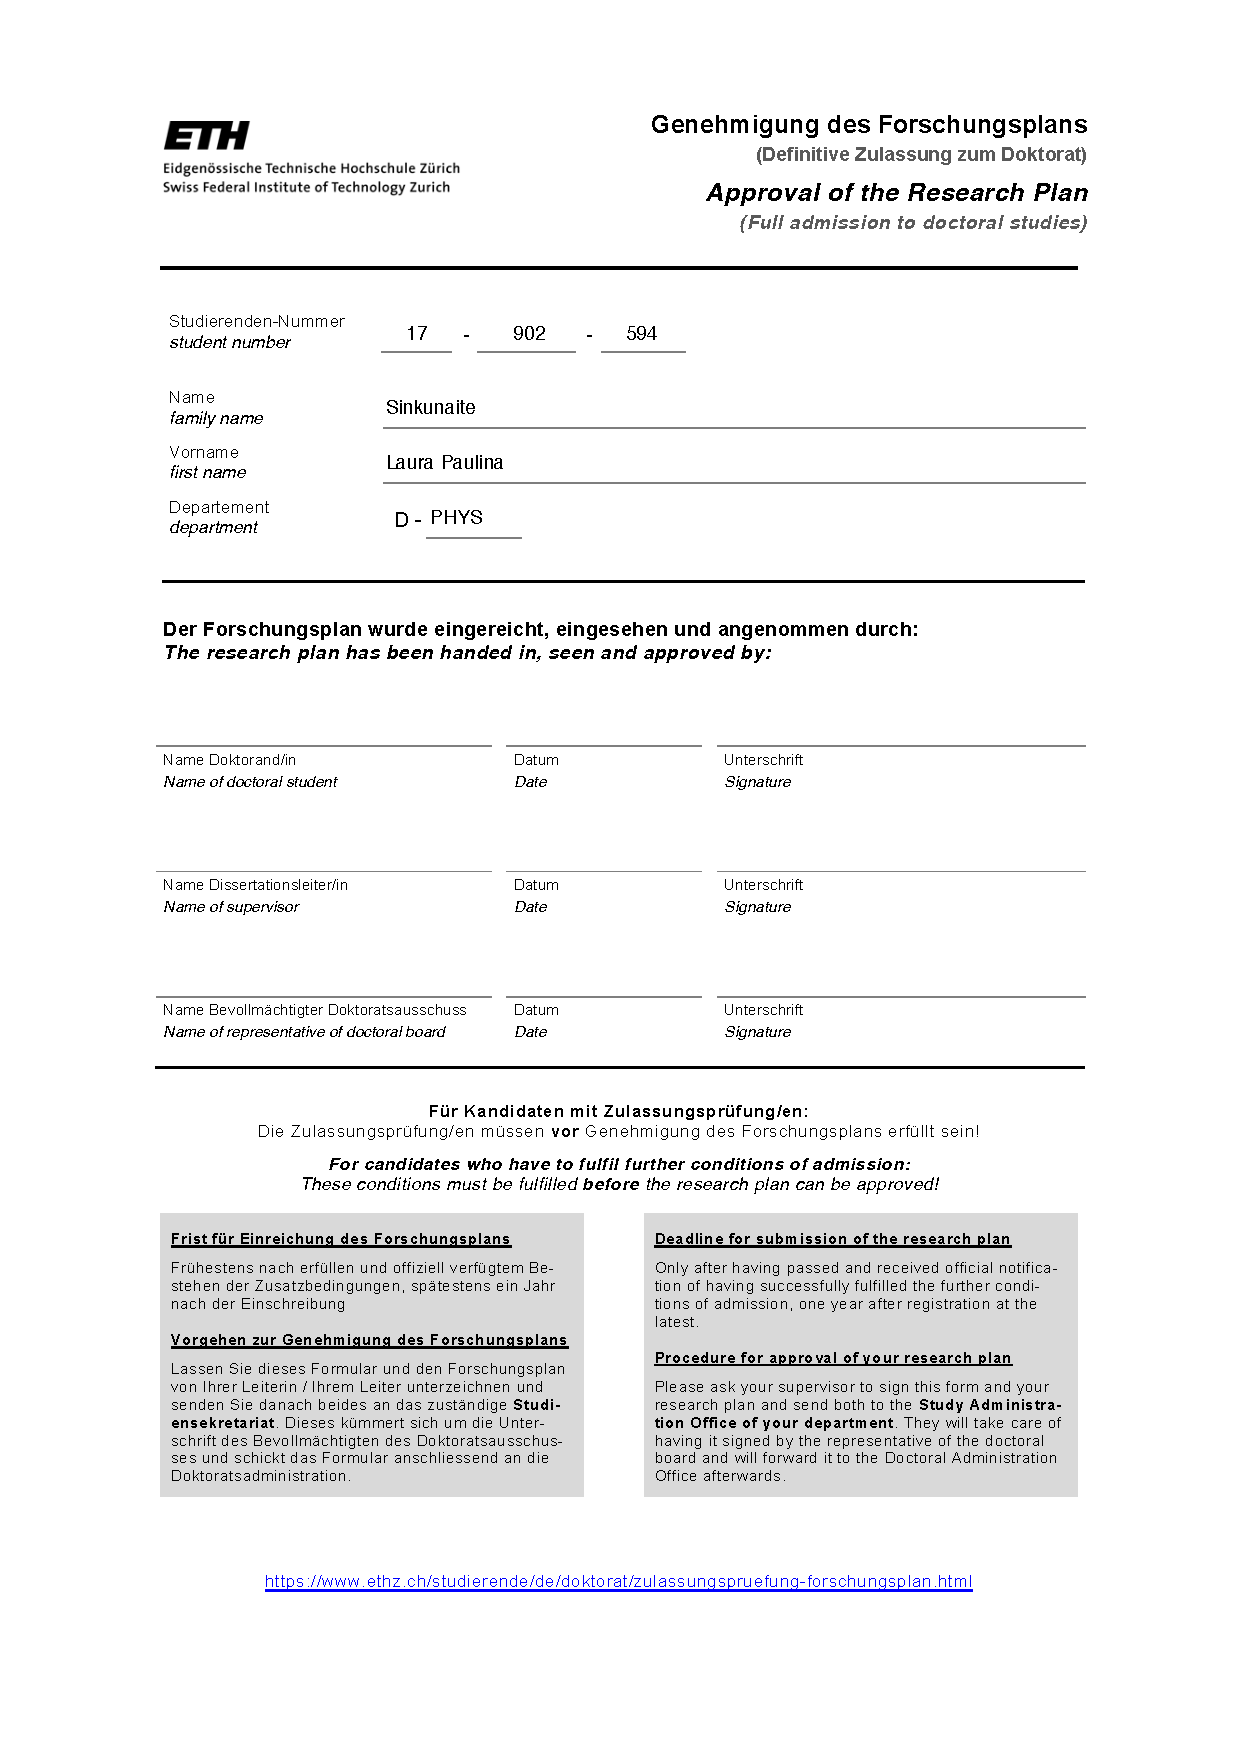
\includepdf[pages=-,pagecommand={},width=\textwidth]{application}
\mbox{}
\thispagestyle{empty}
\newpage
\end{titlepage}
\begin{titlepage}
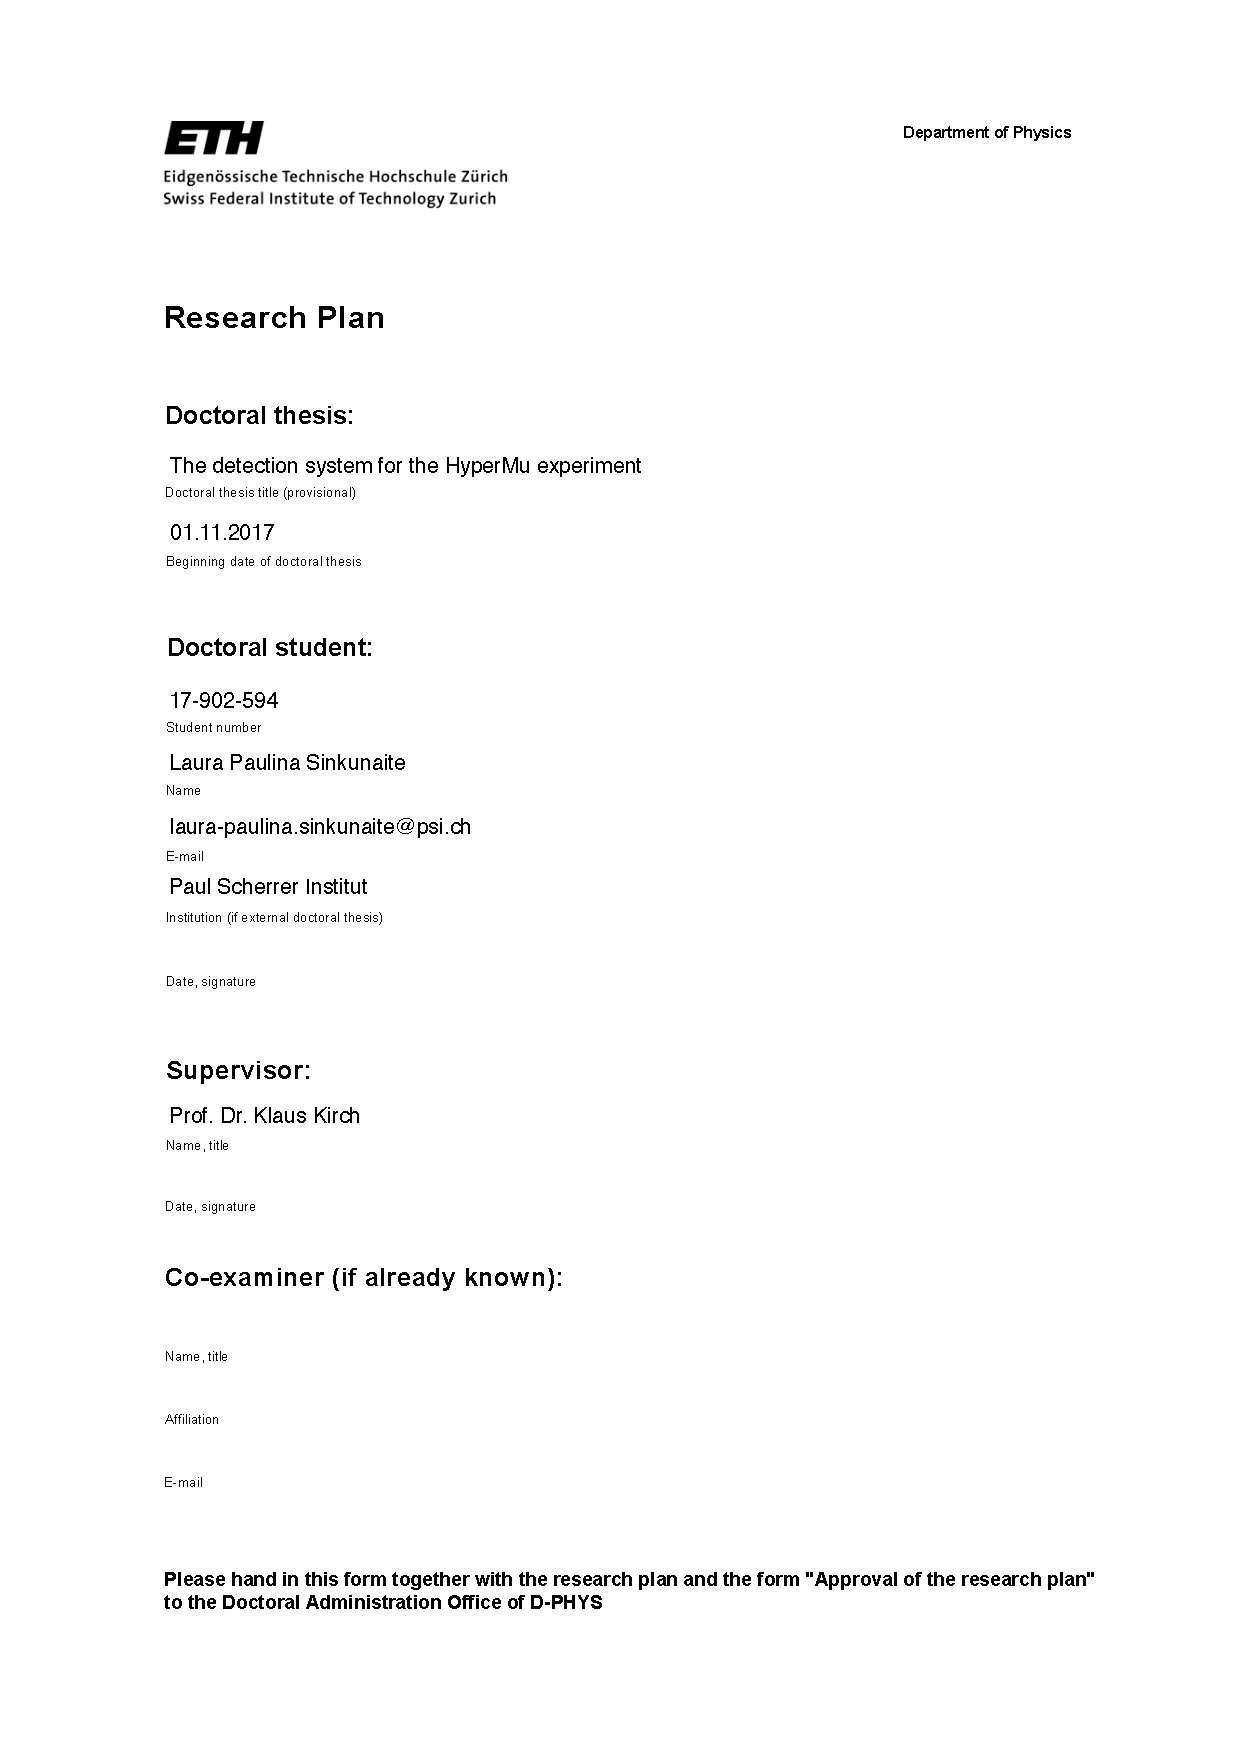
\includepdf[pages=-,pagecommand={},width=\textwidth]{title_page}
\mbox{}
\thispagestyle{empty}
\newpage
\end{titlepage}
%\begin{titlepage}
%
\includepdf[pages=-,pagecommand={},width=\textwidth]{img/title1.pdf}
%\end{titlepage}

% Double-space the manuscript.

\baselineskip24pt

% Make the title.

\maketitle 
\vspace{1.8pt}


% Place your abstract within the special {sciabstract} environment.

%\begin{sciabstract}
 % This document presents a number of hints about how to set up your
%  {\it Science\/} paper in \LaTeX\ .  We provide a template file,
% \texttt{scifile.tex}, that you can use to set up the \LaTeX\ source
%  for your article.  An example of the style is the special
%  \texttt{\{sciabstract\}} environment used to set up the abstract you
%  see here.
%\end{sciabstract}



% In setting up this template for *Science* papers, we've used both
% the \section* command and the \paragraph* command for topical
% divisions.  Which you use will of course depend on the type of paper
% you're writing.  Review Articles tend to have displayed headings, for
% which \section* is more appropriate; Research Articles, when they have
% formal topical divisions at all, tend to signal them with bold text
% that runs into the paragraph, for which \paragraph* is the right
% choice.  Either way, use the asterisk (*) modifier, as shown, to
% suppress numbering.


\section{Introduction and motivation}
\paragraph{Proton-radius puzzle}
The previously conducted measurements \cite{spectroscopy}, \cite{lambshift} of the $2S - 2P$ energy splitting in muonic hydrogen ($\mu{p}$) from the triplet ($2S_{\nicefrac{1}{2}}^{F=1} - 2P_{\nicefrac{3}{2}}^{F=2}$) and the singlet ($2S_{\nicefrac{1}{2}}^{F=0} - 2P_{\nicefrac{3}{2}}^{F=1}$) $2S$ sub-levels have shown a $7{\sigma}$ discrepancy comparing to the values extracted from the electron-proton scattering and hydrogen ($H$) spectroscopy. This so-called ``proton-radius puzzle" is interesting for different areas of physics research: verifications of the proton structure at low energies, new determinations of the Rydberg constant, and searches of BSM physics. Moreover, it has triggered various reanalysis of electron-proton scattering data and several new experiments in the field of scattering and atomic physics. So far, the resolution of the ``proton-radius puzzle'' remains unknown.

\paragraph{Hyperfine splitting}
The Hyperfine splitting (HFS) is the magnetic moment - magnetic moment interaction. This can be described \cite{proposal} as
\begin{equation}
\Delta{E}^{HFS}_{theor} = E^F(1 + {\Delta}_{QED} + {\Delta}_{TPE} + {\Delta}_{weak + HVP}),
\end{equation}
with $E^F$ denoting the Fermi energy
\begin{equation}
E^F = \frac{8}{3}{\alpha}^4 \frac{{\mu}_p{m_1^2}{m_2^2}}{(m_1+m_2)^3},
\end{equation}
${\Delta}_{TPE}$ the two-photon exchange (TPE) contribution (Fig. \ref{fig:tpediagram}), $\alpha$ the fine-structure constant, ${\mu}_p$ the proton magnetic moment, $m_1$ the muon mass, and $m_2$ the proton mass. ${\Delta}_{QED}$ represents the QED contribution, ${\Delta}_{weak+HVP}$ denotes the contribution of hadronic vacuum polarisation and weak interaction, and ${\Delta}_{TPE}$ is the correction due to the proton structure \cite{martynenko}.
\begin{figure}[h]
\centering
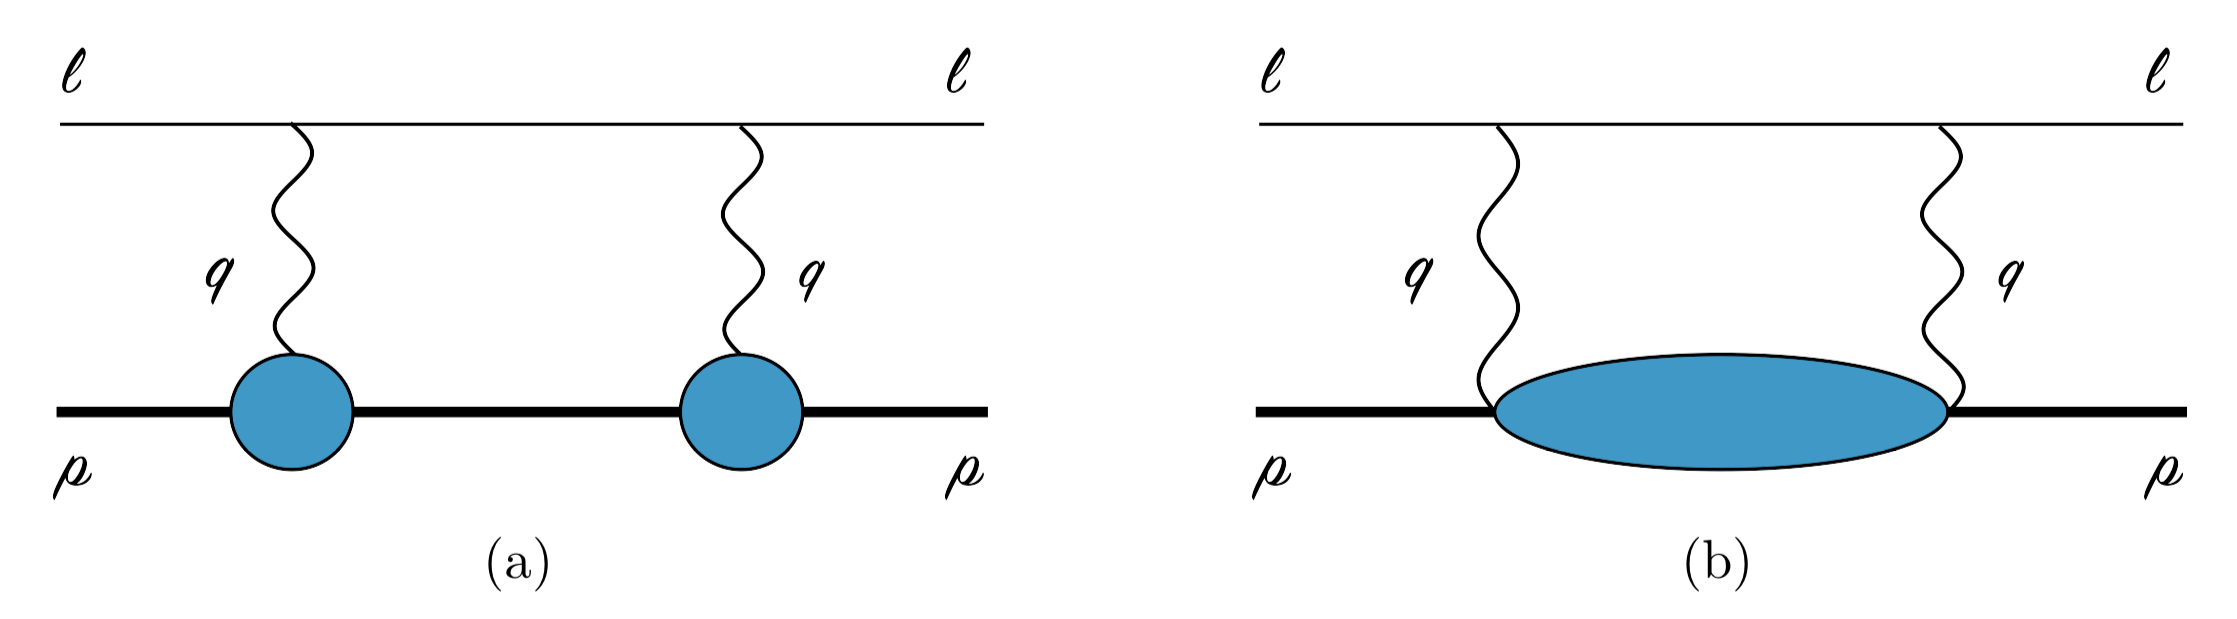
\includegraphics[width=1.0\textwidth]{img/tpediagramms}
\caption{TPE diagrams: the horizontal lines correspond to the lepton and the nucleus (bold). (a) Elastic contribution to the TPE diagram. (b) Inelastic contribution to the TPE diagram, where the "blob" represents all possible excitations \cite{franziska}.}
\label{fig:tpediagram}
\end{figure} 

\paragraph{Two-photon exchange}
The TPE can be divided into $3$ terms,
\begin{equation}
\Delta_{TPE} = \Delta_{Z} + \Delta_{recoil} + \Delta_{pol},
\end{equation}
where the elastic contribution (Zemach) is given by
\begin{equation}
\Delta_{Z} = \frac{8Z{\alpha{m_r}}}{\pi} \int_0^{\infty} \frac{dQ}{Q^2} \Bigg( G_{E}(Q^2) \frac{G_M(Q^2)}{1+\kappa_p} - 1 \Bigg) = -2 (Z{\alpha}) m_r R_Z,
\end{equation}
with the Zemach radius defined as 
\begin{equation}
R_Z = - \frac{4}{\pi} \int_0^{\infty} \frac{dQ}{Q^2} \Bigg( G_E(Q^2) \frac{G_M(Q^2)}{1 + \kappa_p} - 1 \Bigg),
\end{equation}
where ${\kappa}_p$ is a term related to the dipole magnetic moment of the proton. The Zemach radius non-relativistically reduces to the convolution of charge $\rho_{E}$ and magnetic $\rho_{M}$ distributions
\begin{equation}
R_Z = \int d^3 \bm{r} |\bm{r}| \int d^3 \bm{r'} \rho_{E} (\bm{r} - \bm{r'}) \rho_{M} (\bm{r'}).
\end{equation}
This is the contribution with the largest uncertainty of the order of $1 \times 10^{-4}$ of the total HFS. The ${\Delta}_{pol}$ term is the polarisability contribution and the ${\Delta}_{recoil}$ is the negligible recoil correction to the Zemach term. There are two approaches to evaluate the polarisability contribution: using dispersion relations and data such as structure functions and form factors or using chiral perturbation theory. In the dispersive approach, the inelastic contribution can be fully calculated using the measured spin-dependent structure functions of the proton, $g_1(x,Q^2)$ and $g_2(x,Q^2)$ \cite{proposal}.

%The $2S$ Lamb shift, $E_L = \Delta{E}(2S-2P_{\nicefrac{1}{2}})$.\\
%The $2S$ hyperfine splitting, $E_{HFS} = \Delta{E}(2S_{\nicefrac{1}{2}}^{F=1} - 2S_{\nicefrac{1}{2}}^{F=0})$.\\
%The improved value of the proton charge radius $R_E^p = 0.84087(39)$ fm (independent of the HFS prediction).\\
%The Zemach radius of $R_Z^p = 1.082(37)$ fm.\\
%Possible violation of muon-electron universality.\\
%Some possible BSM resolutions: breakdown of the perturbative approach in the electron-proton interaction at short distances, interaction with sea leptons, and unusual proton structure.

\paragraph{Motivation}
The measurement of the $1S-HFS$ transition in the $\mu{p}$ with $1$ ppm accuracy can be used to evaluate the TPE contribution with a relative accuracy of $1 \times 10^{-4}$. This would increase our understanding of the low-energy structure of the proton and would provide a benchmark for chiral perturbation theory, dispersion-based approaches, and lattice QCD. A new experiment (HyperMu) designed to contribute to the resolution of the ``proton-radius puzzle'' is being developed at the Paul Scherrer Institute (PSI). HyperMu is aiming to measure the ground-state hyperfine splitting ($1S - HFS$) in $\mu{p}$ (Fig. \ref{fig:sublevels}) with an accuracy of $1$ ppm by means of laser spectroscopy. From the successful measurement of the $1S-HFS$ transition, the nuclear-structure - related ${\Delta}_{TPE}$ contribution effects can be determined with a relative accuracy of $1 \times 10^{-4}$. In a second step from the TPE, the Zemach radius can be extracted to accuracies of about $\mathcal{O}(10^{-3})$ limited by the theoretical uncertainty of the polarisability contribution. Moreover, the measurement would also be a test of the lepton universality, i.e. when $\mu{p}$ laser spectroscopy results are compared to the electron-proton scattering and to the electronic hydrogen ($ep$) spectroscopy, and on top of that it would impact the resolution of the ``proton radius puzzle'' and the related ``new physics'' searches. 
\begin{figure}[h]
\centering
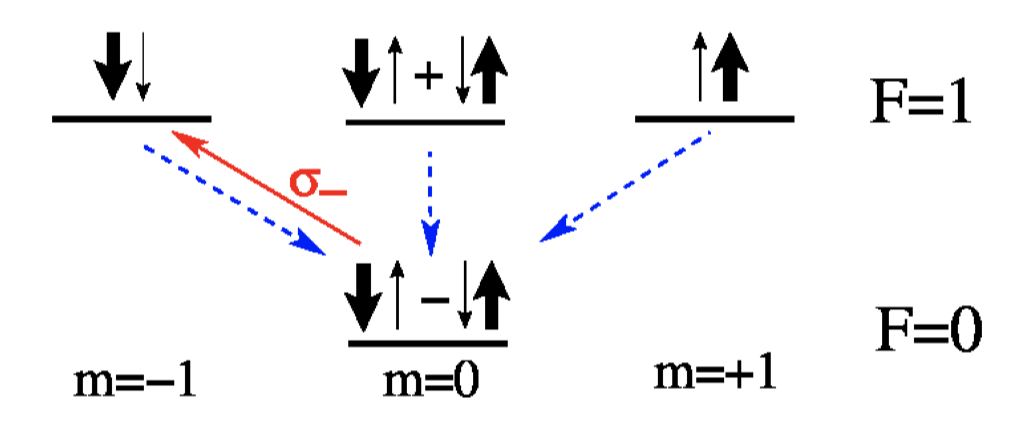
\includegraphics[width=0.7\textwidth]{img/sublevels}
\caption{Energy levels and spin compositions of the $1S$ states in $\mu{p}$. The red arrow represents the transition driven by the circularly polarised laser light, the blue arrows illustrate the collisional quenching \cite{proposal}.}
\label{fig:sublevels}
\end{figure}
%\vspace{3.8pt}

%(1) bound-state QED test of the 1S-HFS in H: understanding the $21$ cm line, (2) understanding of the proton structure, (3) nuclear physics from ${\mu}^3He^+$.
%Fundamental to all the constants. 
%Development of novel laser technologies.

%\newpage
\section{Working principle}
\paragraph{The principle of the HyperMu experiment:}
Muons are stopped in hydrogen gas forming ${\mu}p$ atoms in highly-excited states. The formed ${\mu}p$ atoms de-excite to the $F=0$ sub-level of the ground state (Fig. \ref{fig:sublevels}). A high-energy laser pulse ($3$ mJ at $6.7 {\mu}m$ and $100$ MHz bandwidth) excites the ${\mu}p$ atoms to the $F=1$ sub-level of the ground state,
%\begin{enumerate}
%\item
%Formation: a muon is stopped in hydrogen gas forming a ${\mu}p$ atom in a highly excited state.
%\item
%De-excitation: the formed ${\mu}p$ atom de-excites to the $F=0$ sub-level of the ground state.
%\item
%Laser excitation: a high-energy laser pulse excites the ${\mu}p$ atom,
\begin{equation*}
{\mu}p_{F=0} + {\gamma} \rightarrow {\mu}p_{F=1}.
\end{equation*}
In collisions with hydrogen molecules ($H_2$), the $\mu{p}$ atoms are de-excited to the $F=0$ sub-level,
%\item
%Collisional de-excitation: in a collision with a hydrogen molecule ($H_2$), the ${\mu}p$ atom is de-excited to the $F=0$ sub-level of the ground state and after ${\sim}1$ ${\mu}s$ is thermalised to the hydrogen gas temperature ($50$ K),
\begin{equation*}
{\mu}p_{F=1} + H_2 \rightarrow {\mu}p_{F=0} + H_2 + E_{kin}.
\end{equation*}
This transition energy is converted into the kinetic energy. Having this extra kinetic energy, the ${\mu}p$ atoms efficiently diffuse to the target walls before muon decays occur. At the target wall, which is made of the high-Z material, the muons are transferred from the $\mu{p}$ to the high-Z material forming $({\mu}Z)^{*}$ in an excited state. The highly-excited $({\mu}Z)^{*}$ atoms then de-excite producing MeV X-rays. The MeV X-rays are detected using scintillating detectors (Fig. \ref{fig:targetscheme}). A resonance curve is obtained by plotting the number of the X-rays versus the laser frequency. 
%\item
%Diffusion: having this extra kinetic energy, the ${\mu}p$ atom efficiently diffuses to the target walls before muon decay occurs.
%\item
%At the wall: at the target wall, which is made of high-Z material, the muon is transferred from the muonic hydrogen to the high-Z material forming $({\mu}Z)^*$ in an excited state. The highly excited $({\mu}Z)^*$ atoms then de-excite producing MeV X-rays.
%\item
%Detection: the MeV X-rays are detected using scintillators. A resonance is obtained by plotting the number of X-rays versus the laser frequency.
%\end{enumerate}
\begin{figure}[h]
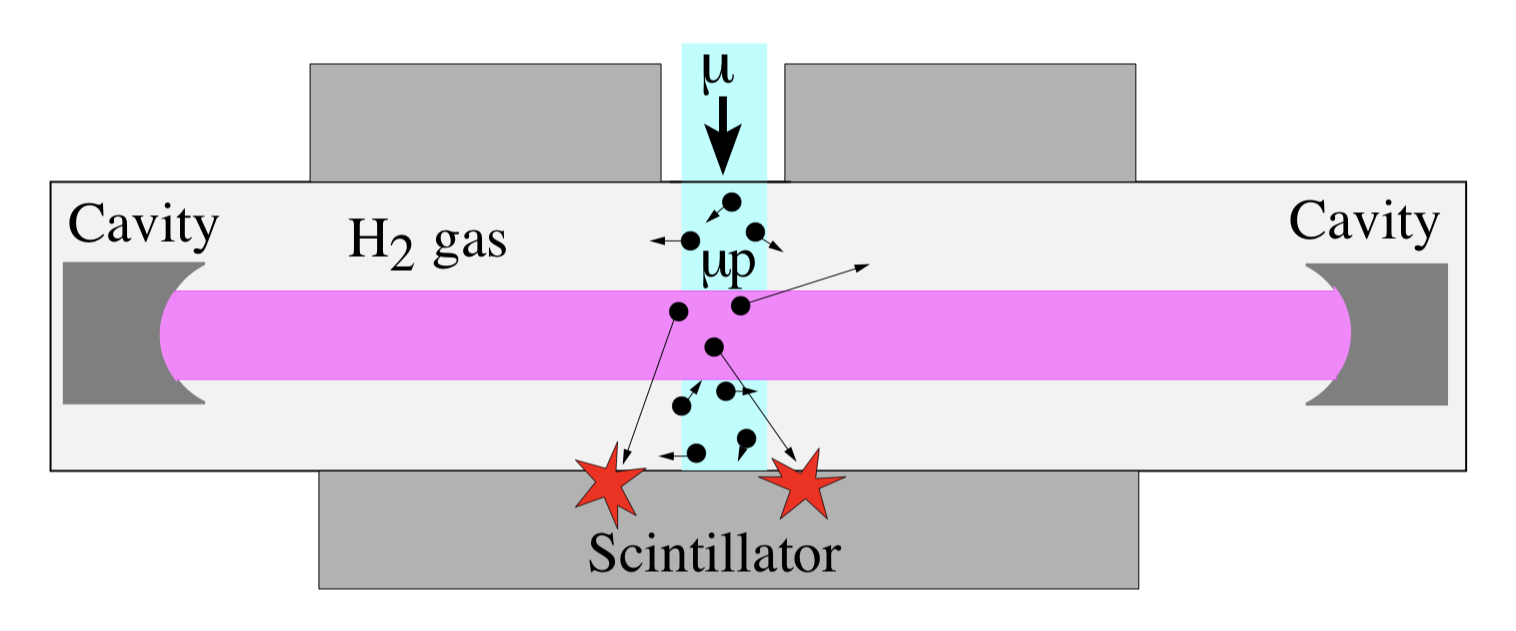
\includegraphics[width=1.0\textwidth]{img/targetscheme}
\caption{HyperMu experimental scheme showing a laser cavity, muon entrance beam, and the surrounding scintillating detectors \cite{proposal}.}
\label{fig:targetscheme}
\end{figure}



\paragraph{Signal and background}\label{para:signature}
The signal events are considered to be the MeV X-rays detected within a time window ${\Delta}t$ after the laser excitation. There are two types of background events: intrinsic and erroneous. The intrinsic background is produced by non-laser excited ${\mu}p$ atoms, that diffuse to the target walls in the observation time window ${\Delta}t$. This type of background can be minimised by cooling down the target, e.g. keeping the $H_2$ gas at $50$ K temperature. The other type of background arises from the electrons produced in the event of a muon decay, ${\mu}^- \rightarrow e^- + \overline{{\nu}_e} + {\nu}_{\mu}$, and being falsely identified as X-rays. 
%\begin{itemize}
%\item
%Signal: MeV X-rays detected in a time window ${\Delta}t$ after the laser excitation.
%\item
%Intrinsic background: produced by non-laser excited ${\mu}p$ atoms, that diffuse to the target walls in the observation time window ${\Delta}t$. Cosmics.
%\item
%Other backgrounds: caused by electrons from muon decays falsely identified as X-rays.
%\end{itemize}
%It is bad if an electron is identified as an X-ray. We need to minimise this erroneous background to manage having enough statistics for the successful run of the experiment. 

\paragraph{Laser system}
To produce a resonance curve for the $1S - HFS$ transition in the $\mu{p}$, a high-energy laser system delivering $3$ mJ pulses with $100$ MHz bandwidth at $6.7$ ${\mu}m$ is needed. We are planning to realise a laser system as depicted in Fig. \ref{fig:opopascheme}. It is composed of a thin-disk laser followed by optical-parametric down-conversion stages (OPO - OPA) and a difference frequency generating stage (DFG). Using this OPO and OPA scheme, the thin-disk laser needs to be operated in single-frequency mode achieved by injection seeding the thin-disk laser oscillator with an external frequency stabilised continuous-wave (cw) laser at $1030$ nm. The pulses at $1030$ nm would then be down-converted in a non-linear crystal to produce two beams, so called an ``idler'' beam at $2434$ nm and a ``signal'' beam at $1785$ nm. The OPO cavity needs to be seeded by a tunable ``signal'' laser used to scan the resonance. A successive difference frequency generation (DFG) between ``idler'' and ``signal'' pulses would then be used to generate $3$ mJ pulses at $6.7 {\mu}$m. 
\begin{figure}[h]
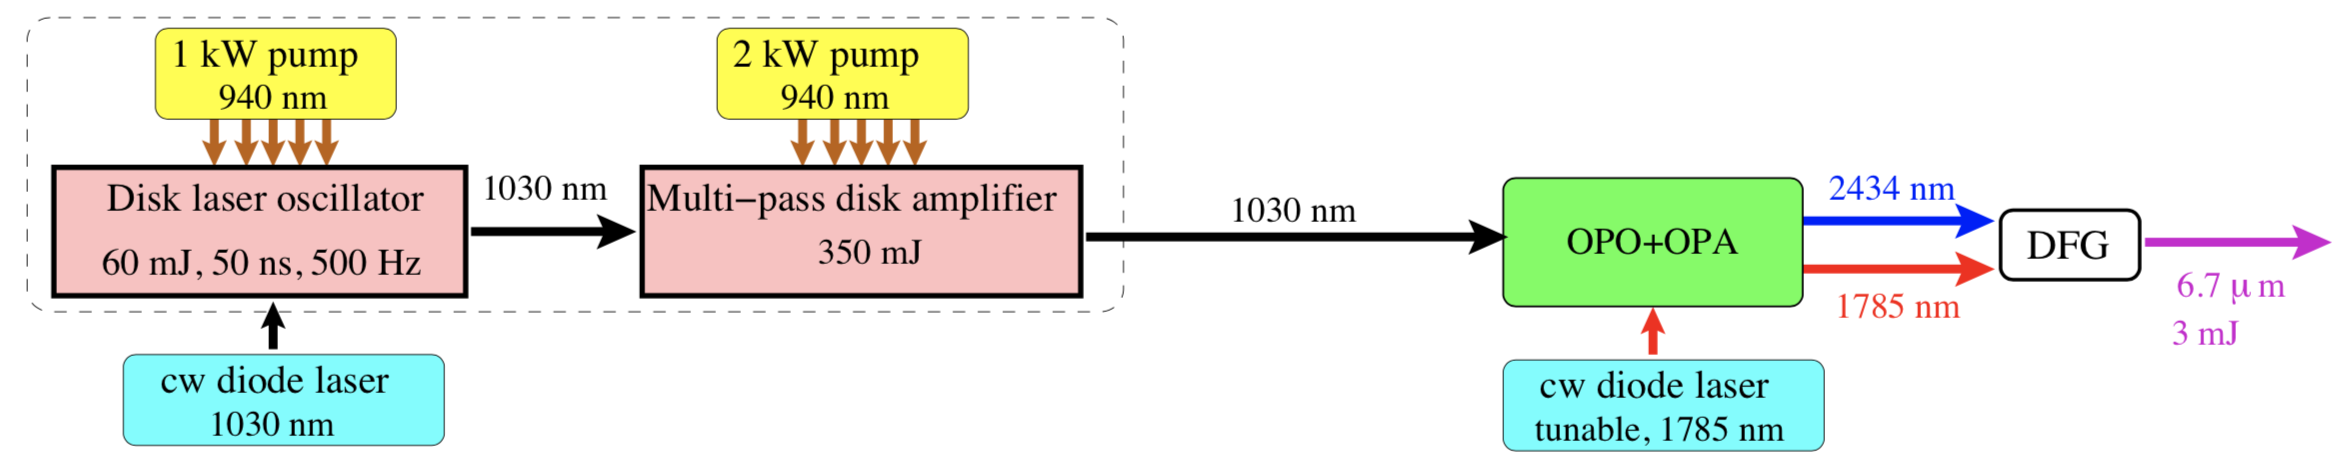
\includegraphics[width=1.0\textwidth]{img/OPOschemeOPA}
\caption{Possible parametric down-conversion laser scheme for $\mu{p}$ experiment using OPO and OPA technologies \cite{proposal}.}
\label{fig:opopascheme}
\end{figure}


\section{The detection system}
\paragraph{Requirements}
One of the main topics of this thesis is to develop the needed detection system for the HFS experiment. The aims of the detection system are listed below.
\begin{enumerate}
\item
	Detection of the incoming muons. The detected signal is used to trigger the Data Acquisition (DAQ) and the laser systems. 
\item
	Measurement of the produced X-ray cascades in the $({\mu}Z)^*$ de-excitation process after the ${\mu}p$ atoms have diffused to the target wall.
\item
	Detection of the nuclear capture event. After de-excitation to the ground-state, the muons in the ${\mu}Z$ atoms are mainly captured in the nuclear process (${\mu}^- + p \rightarrow n + {\nu}_{\mu}$).
\item
	The detection system also needs to measure the electrons from regular muon decays. Those electrons are produced mainly by the ${\mu}p$ atoms formed in the hydrogen gas that decay have not reached the target wall. Note that the nuclear capture rate in the ${\mu}p$ atom is much smaller than in high-$Z$ ${\mu}Z$ atoms. 
\item
	The detection system must also deal with the background coming from the beam-line and muons stopping in the entrance detector and target window.
\end{enumerate}
For simplicity, in this plan we will only describe the detection of electrons coming from the muon decays and X-rays coming from the muonic X-ray cascade (Table \ref{table:cascade}).
%\begin{figure}[!htbp]
%\centering
%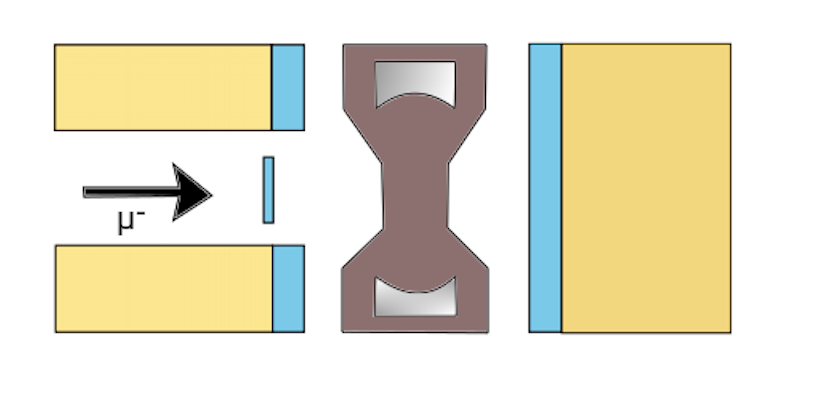
\includegraphics[width=0.8\textwidth]{img/setup2.png}
%\caption{Sketch of the detection system. After the incoming muon beam hits the entrance detector (shown in blue), it enters the target area (brown) with the thoroidal cavity inside (grey). On both down-stream and up-stream parts, series of different thickness plastic scintillators are going to be used (yellow and blue) to detect the X-ray signal and to distinguish it from the background.}
%\label{fig:setup}
%\end{figure}


\paragraph{Detectors}
The ideal detector for measuring the muonic X-rays would be germanium (Ge) as it provides an excellent energy resolution. However, its detection rate (possible solid angle coverage) is too low for HyperMu. Therefore, we need to use alternative detectors that could fulfil the following conditions.
\begin{enumerate}[i.]
\item
High detection efficiency for cascade ($\geq 50\%$) and electron, and the ability to distinguish between them (the false identification of electrons as X-rays should be $< 5 \times 10^{-3}$). Time resolutions must be of about $10$ ns. We are considering to use thin plastic scintillators to distinguish between X-ray from the cascade event and an electron from the muon decay (Fig. \ref{fig:energy_cut}). The energy spectrum of cascade events differs considerably from the energy spectrum of an electron from muon decay. 
\item
Indeed, during a cascade process several X-rays are produced (see Table \ref{table:cascade}) with total energy of about $10$ MeV. Since only a fraction of these X-rays (and energy) is detected in the scintillator, a complex measurable energy spectrum is obtained with an ``endpoint" energy of $10$ MeV (see Fig. 7). Therefore, a simple energy cut could be used to partially sort out between $e^-$ and X-rays. 
\end{enumerate}
The energy spectrum of the emitted electron from muon decay is shown in Fig. \ref{fig:michel}. Electrons up to the energies of $50$ MeV are emitted in the muon decay. A considerable fraction is above $10$ MeV. So these events which deposit more than $10$ MeV energy in the scintillator can be identified as ``electrons''. Therefore, a simple energy cut could be used to partially sort out between $e^-$ and X-rays.
\begin{table}[htpb]
\caption{X-ray transitions in gold}
\centering
\begin{tabular}{c c c}
\hline\hline
Transition $n_i \rightarrow n_j$ & Relative probability [$\%$] & Energy [MeV]\\ [0.5ex]
\hline
$2 \rightarrow 1$ & 90.00 & 5.65 \\
$3 \rightarrow 1$ & 4.50 & 8.10 \\
$4 \rightarrow 1$ & 0.30 & 9.00 \\
$5 \rightarrow 1$ & 0.10 & 9.40 \\
$>6 \rightarrow 1$ & 1.00 & 9.60 \\ [0.5ex]
\hline
$3 \rightarrow 2$ & 84.00 & 2.40 \\
$4 \rightarrow 2$ & 6.00 & 3.30 \\
$5 \rightarrow 2$ & 1.11 & 3.70 \\
$6 \rightarrow 2$ & 0.40 & 3.90 \\
$>7 \rightarrow 2$ & 0.25 & 4.20 \\ [0.5ex]
\hline
$4 \rightarrow 3$ & 76.00 & 0.90 \\
$5 \rightarrow 3$ & 8.00 & 1.30 \\
$6 \rightarrow 3$ & 2.00 & 1.50 \\
$7 \rightarrow 3$ & 0.80 & 1.70 \\
$>8 \rightarrow 3$ & 2.50 & 1.80 \\ [0.5ex]
\hline
$5 \rightarrow 4$ & 66.00 & 0.40 \\
$6 \rightarrow 4$ & 9.00 & 0.60 \\
$7 \rightarrow 4$ & 3.00 & 0.70 \\
$8 \rightarrow 4$ & 1.00 & 0.85 \\
$>9 \rightarrow 4$ & 4.00 & 0.90 \\ [0.5ex]
\hline
$6 \rightarrow 5$ & 64.00 & 0.22 \\
$7 \rightarrow 5$ & 11.00 & 0.36 \\
$8 \rightarrow 5$ & 3.00 & 0.45 \\
$9 \rightarrow 5$ & 1.50 & 0.52 \\
$>10 \rightarrow 5$ & 5.00 & 0.55 \\ [0.5ex]
\hline
$7 \rightarrow 6$ & 62.00 & 0.13 \\
$8 \rightarrow 6$ & 12.00 & 0.22 \\
$9 \rightarrow 6$ & 4.00 & 0.29 \\
$10 \rightarrow 6$ & 2.00 & 0.33 \\
$>11 \rightarrow 6$ & 6.00 & 0.36 \\ [1ex]
\hline
\end{tabular}
\label{table:cascade}
\end{table}
\begin{figure}[ht!]
\centering
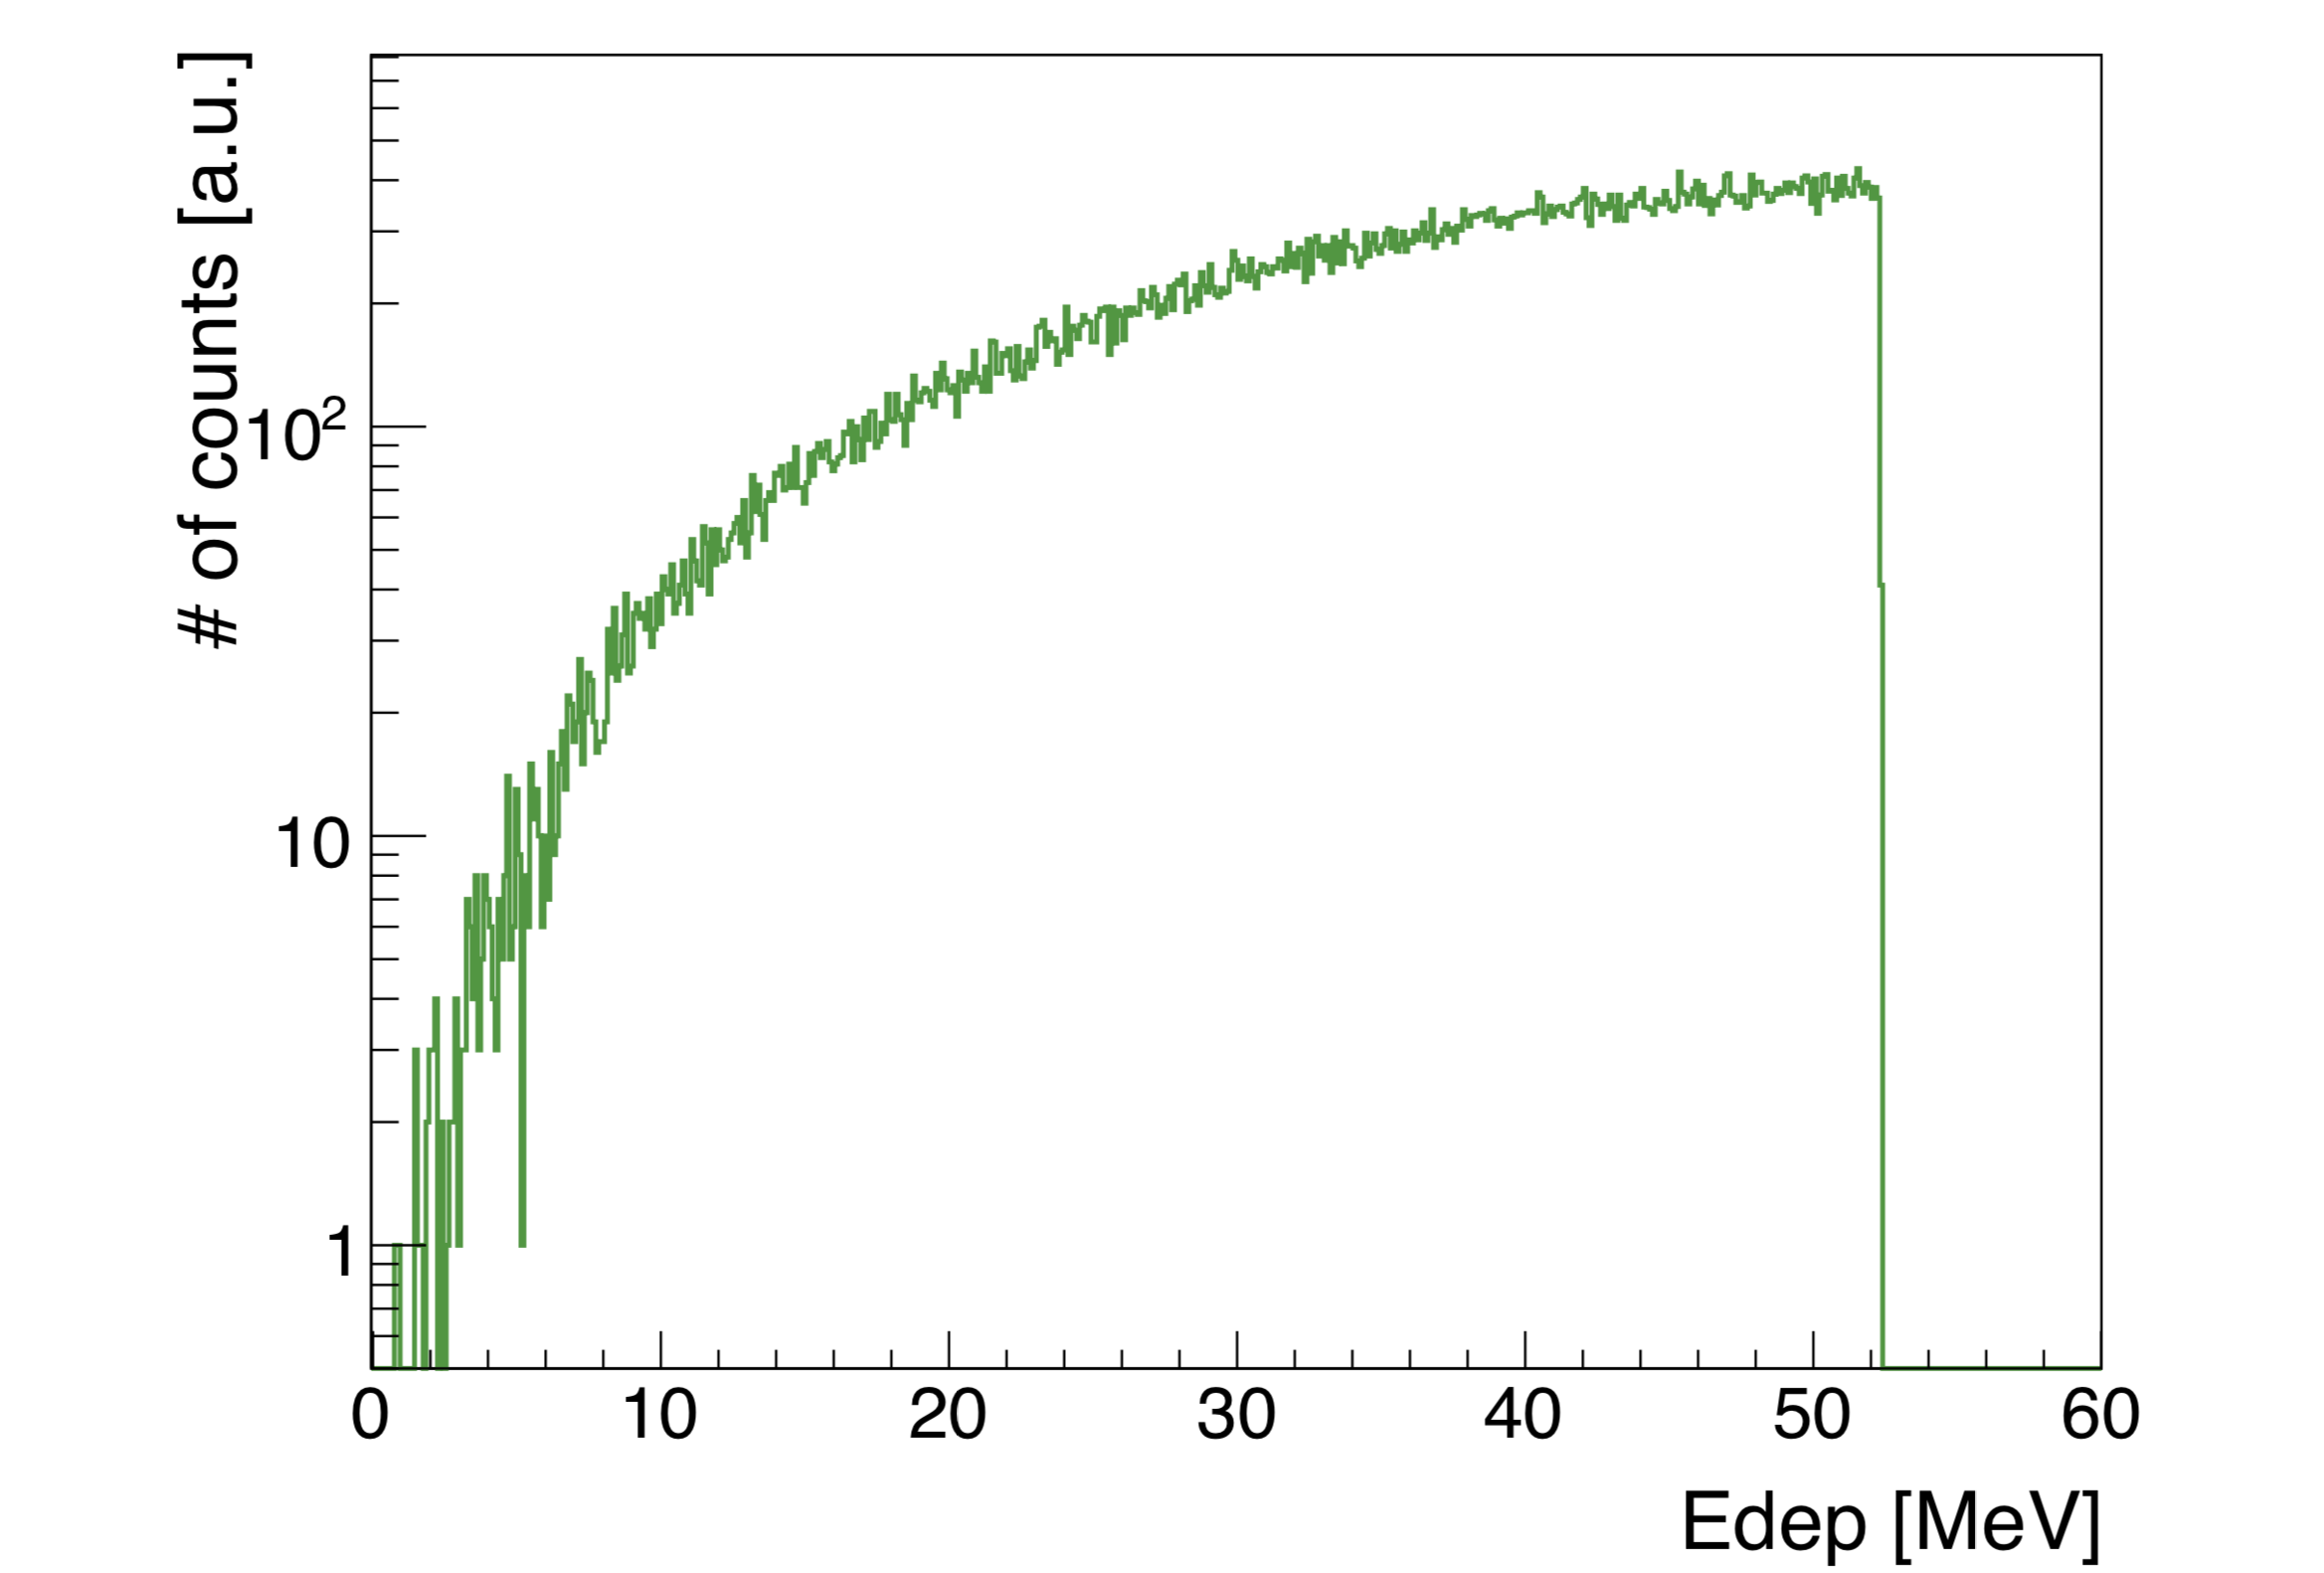
\includegraphics[width=0.6\textwidth]{img/michel}
\caption{Michel decay spectrum for a muon.}
\label{fig:michel}
\end{figure}
%\begin{figure}[ht!]
%\centering
%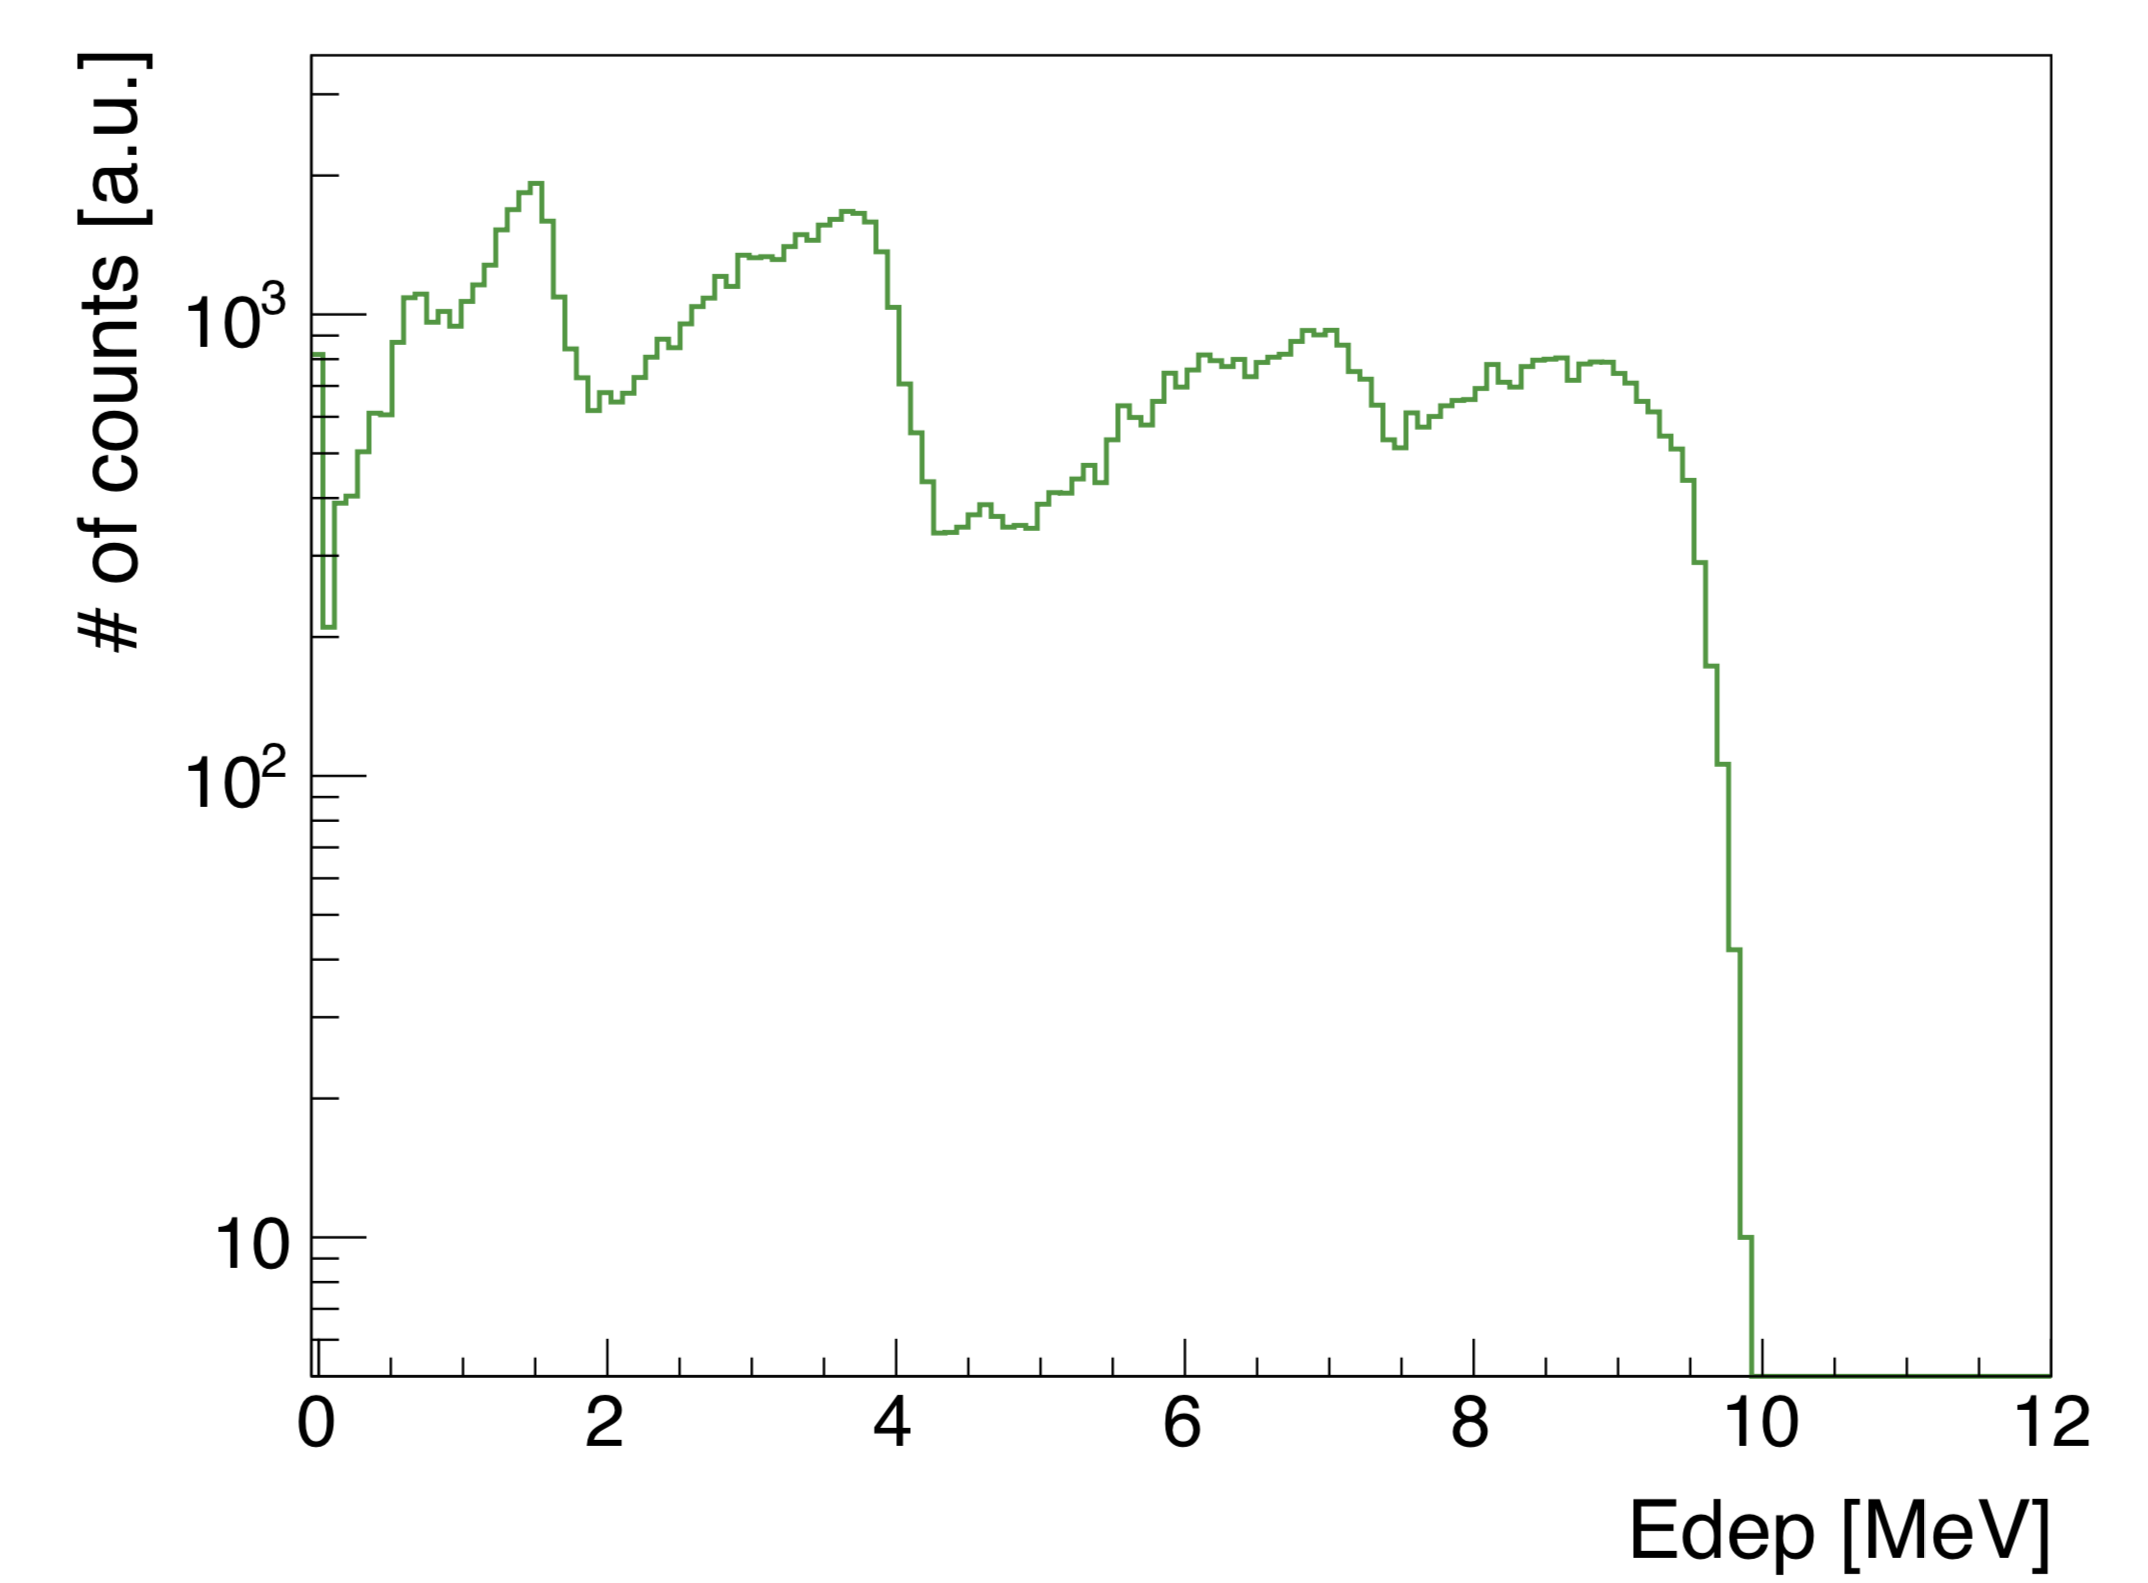
\includegraphics[width=0.65\textwidth]{img/cascade}
%\caption{Deposited energy of the X-ray cascade in the $5$-mm thick plastic scintillator.}
%\label{fig:cascade}
%\end{figure}

\paragraph{Signal to background ratio}
%\begin{figure}[!htbp]
%\centering
%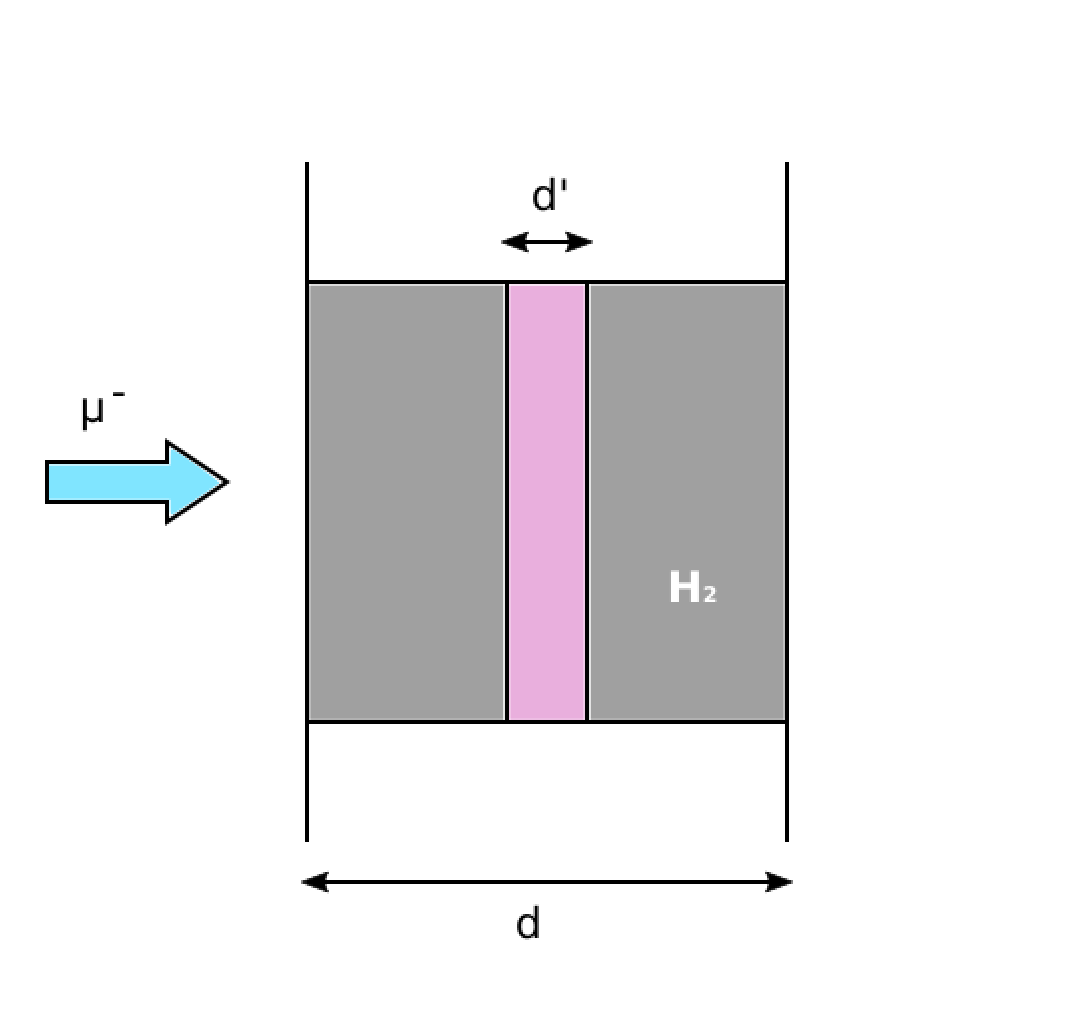
\includegraphics[width=0.6\textwidth]{img/sig2bkg.png}
%\caption{Signal to background ratio.}
%\label{fig:sig2bkg}
%\end{figure}
In this sub-section we briefly motivate the requirements that the false identification of $e^-$ as cascade events should have a probability smaller than $5 \times 10^{-3}$. This requirement can be estimated by calculating the number of ${\mu}p$ atoms which are in the hydrogen gas target and decay in the event time window $\Delta{t} \sim 300$ ns following the laser excitation, and by comparing it to the number of $\mu{p}$ atoms that after the laser-excitation reach the target walls in the observation time window $\Delta{t}$. Then the number of muon decay in the observation time window $\Delta{t} = 300$ ns (see Fig. \ref{fig:diffusion}) can be expressed as
\begin{equation}
B \approx d \Big(\frac{A_2}{A_1}\Big)  N_{stopped\: {\mu}^-} P_{{\mu}^- \rightarrow {e^-}\overline{{\nu}_e}{\nu}_{\mu}} \varepsilon_{det, e^-} = d \Big(\frac{A_2}{A_1}\Big) N_{stopped\: {\mu}^-}  \Bigg(1 - e^{-\frac{300 ns}{2200 ns}}\Bigg) \varepsilon_{det,e^-},
\end{equation}
where d is the target length, the ratio $\frac{A_2}{A_1}$ represents the $\mu{p}$ density loss in the time between the muonic atom formation and the base excitation, $P_{{\mu}^- \rightarrow {e^-}\overline{{\nu}_e}{\nu}_{\mu}}$ is the probability for a muon to decay and produce an electron, and $\varepsilon_{det}$ is the detection probability of such an event. The signal, $S$, on the other hand, can be expressed as
\begin{equation}
S \approx d' \Big(\frac{A_2}{A_1}\Big) N_{stopped\: {\mu}^-} P_{laser-excited} P_{laser-excited\: reach\: the\: wall} \varepsilon_{det, X}.
\end{equation}
Here, $d'$ is the width of the laser-excited region, $P_{laser-excited}$ is the probability that the atoms in the region get excited by the laser, $P_{laser-excited\: reach\: the\: wall}$ is the probability that those that had been laser-excited will reach the wall of the target. Now, if we calculate the signal-to-background ratio, some of the parameters approximately cancel out:
\begin{equation}
\frac{S}{B} \approx \Big(\frac{d'}{d}\Big) \Big(\frac{\varepsilon_{det,X}}{\varepsilon_{det,e^-}}\Big) \frac{{P_{laser-excited}}{P_{laser-excited\: reach\: the\: wall}}}{ \Big(1 - e^{-\frac{300ns}{2200ns}}\Big)} = \Big(\frac{d'}{d}\Big)\Big(\frac{\varepsilon_{det,X}}{\varepsilon_{det,e^-}}\Big) \frac{P_{laser}}{\Big(1 - e^{-\frac{300ns}{2200ns}}\Big)},
\end{equation}
where $\frac{d'}{d}$ is the so-called overlap region, $P_{laser}$ is a combined probability that the muonic atom will be laser excited and will reach the wall, and it is equal to $\sim 1 \%$. Thus, the ratio $\frac{S}{B}$ is approximately $5 \times 10^{-3}$.
\begin{figure}[!htbp]
\centering
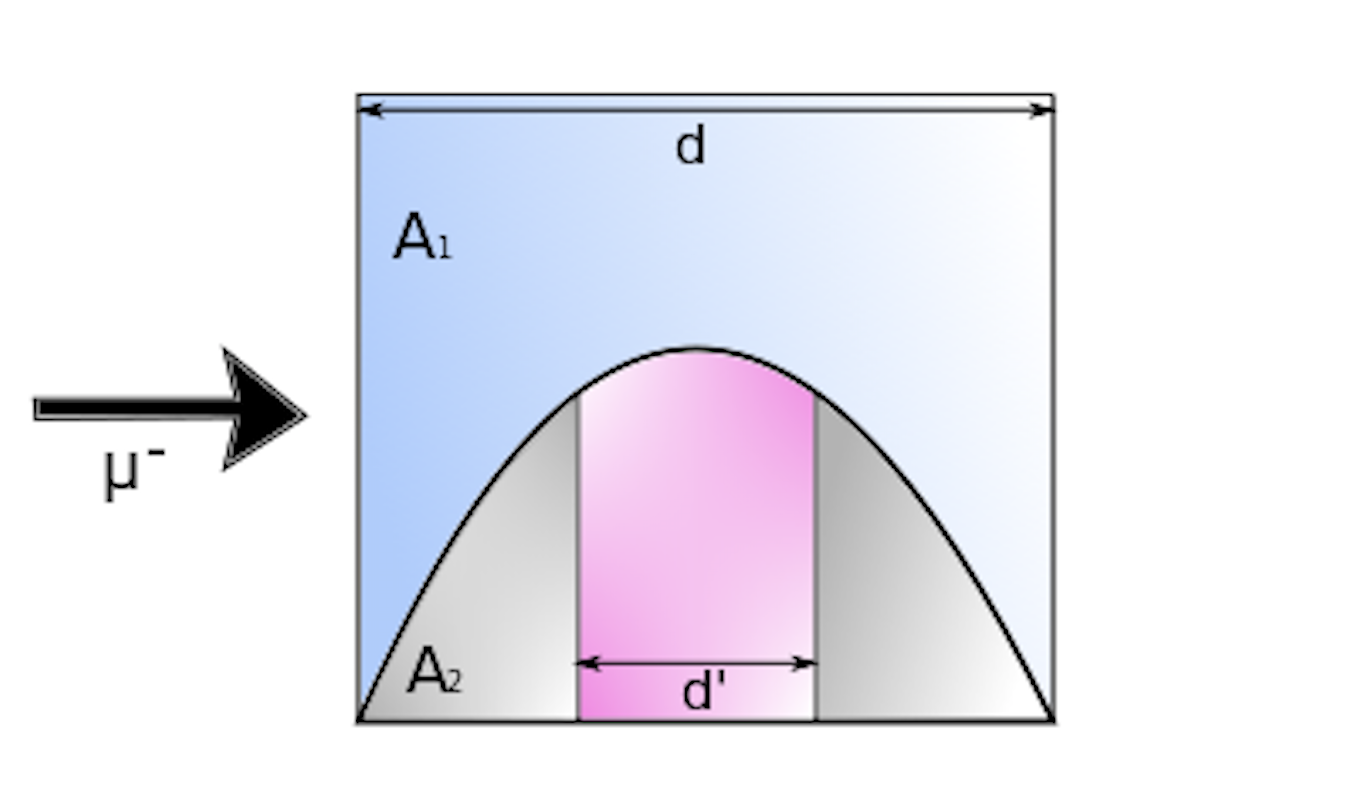
\includegraphics[width=0.7\textwidth]{img/diffusion2.png}
\caption{The density distribution of the $\mu{p}$ atoms in the target. The $x$-axis points to the right and it represents the beam direction, whereas the $y$-axis is pointing downwards representing the time scale. The blue area $A_1$ shows the situation at the time $t = 0$ ns. The almost parabolic grey area $A_2$ marks the loss normalisation background at the time when the laser enters the cavity $t = 1000$ ns, whereas the pink region depicts the loss normalisation signal at the time $t = 1000$ ns $ + t_{excitation}$.}
\label{fig:diffusion}
\end{figure}

\paragraph{Combination of thin and thick scintillators}
Electrons and X-rays also can be partially distinguished by considering their total deposited energy. In fact, cascade events have energies up to $10$ MeV while the energies of the electrons from the muon decay are distributed according to Fig. \ref{fig:michel}. A thick scintillator that completely absorbs the X-rays and the electrons could be used. A thin scintillator placed in front of the thick scintillator can be used to further distiguish between $e^-$ and cascade events. Figure X shows the energy spectrum for cascade and $\mu$-decay events in a $5$-mm thick scintillator. By introducing an energy cut between $0.5 - 1$ MeV, we can distinguish between cascade and $e^-$ events. 
\begin{figure}[!htbp]
\begin{subfigure}{.485\textwidth}
	\centering
	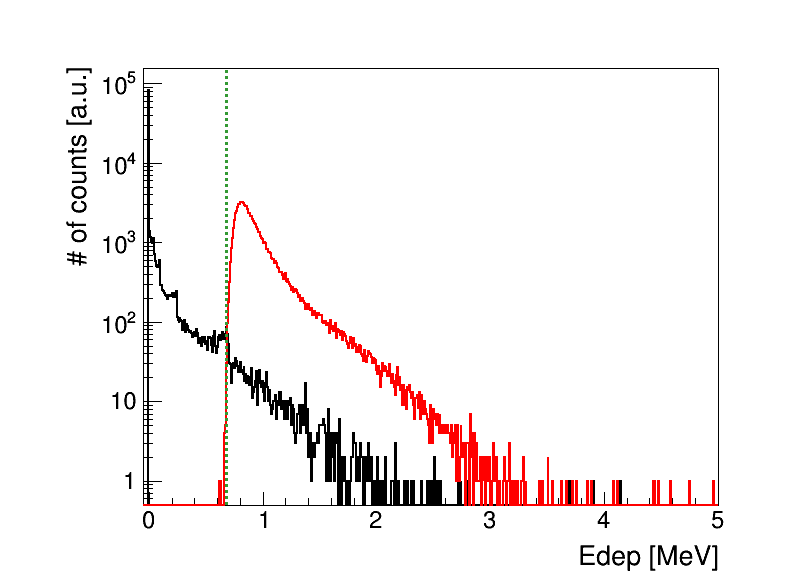
\includegraphics[width=0.97\textwidth]{img/researchplan_5mm_separation.png}
	\subcaption{Deposited energy in the $5$-mm light plastic scintillator. A lower energy cut at $0.7$ MeV [green dashed line] marks the intersection of different energy profiles and allows us to partially distinguish between the particles.}
	\label{fig:sep_5mm}
\end{subfigure}\hspace*{4.5mm}
\begin{subfigure}{.485\textwidth}
	\centering
	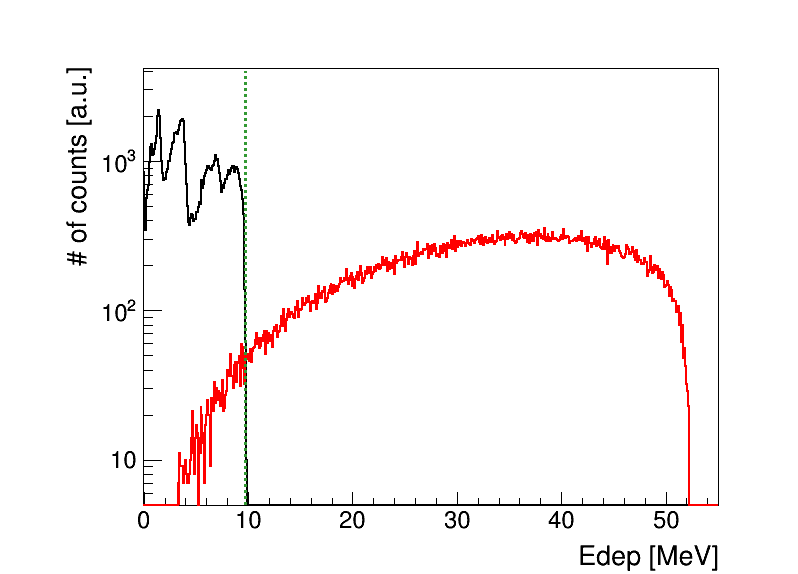
\includegraphics[width=0.97\textwidth]{img/researchplan_250mm_separation}
	\subcaption{Deposited energy in the $250$-mm light plastic scintillator. An upper energy cut at $10$ MeV [green dashed line] marks the intersection of different energy profiles and allows us to partially distinguish between the particles.}
	\label{fig:sep_250mm}
\end{subfigure}	
\caption{Deposited energy differences between electrons [red] and X-rays [black] in the $5$-mm and $250$-mm light plastic scintillator. The green dashed line shows a possible location for a cut to distinguish X-rays from electrons.}
\label{fig:energy_cut}
\end{figure}

%\begin{figure}[ht!]
%\centering
%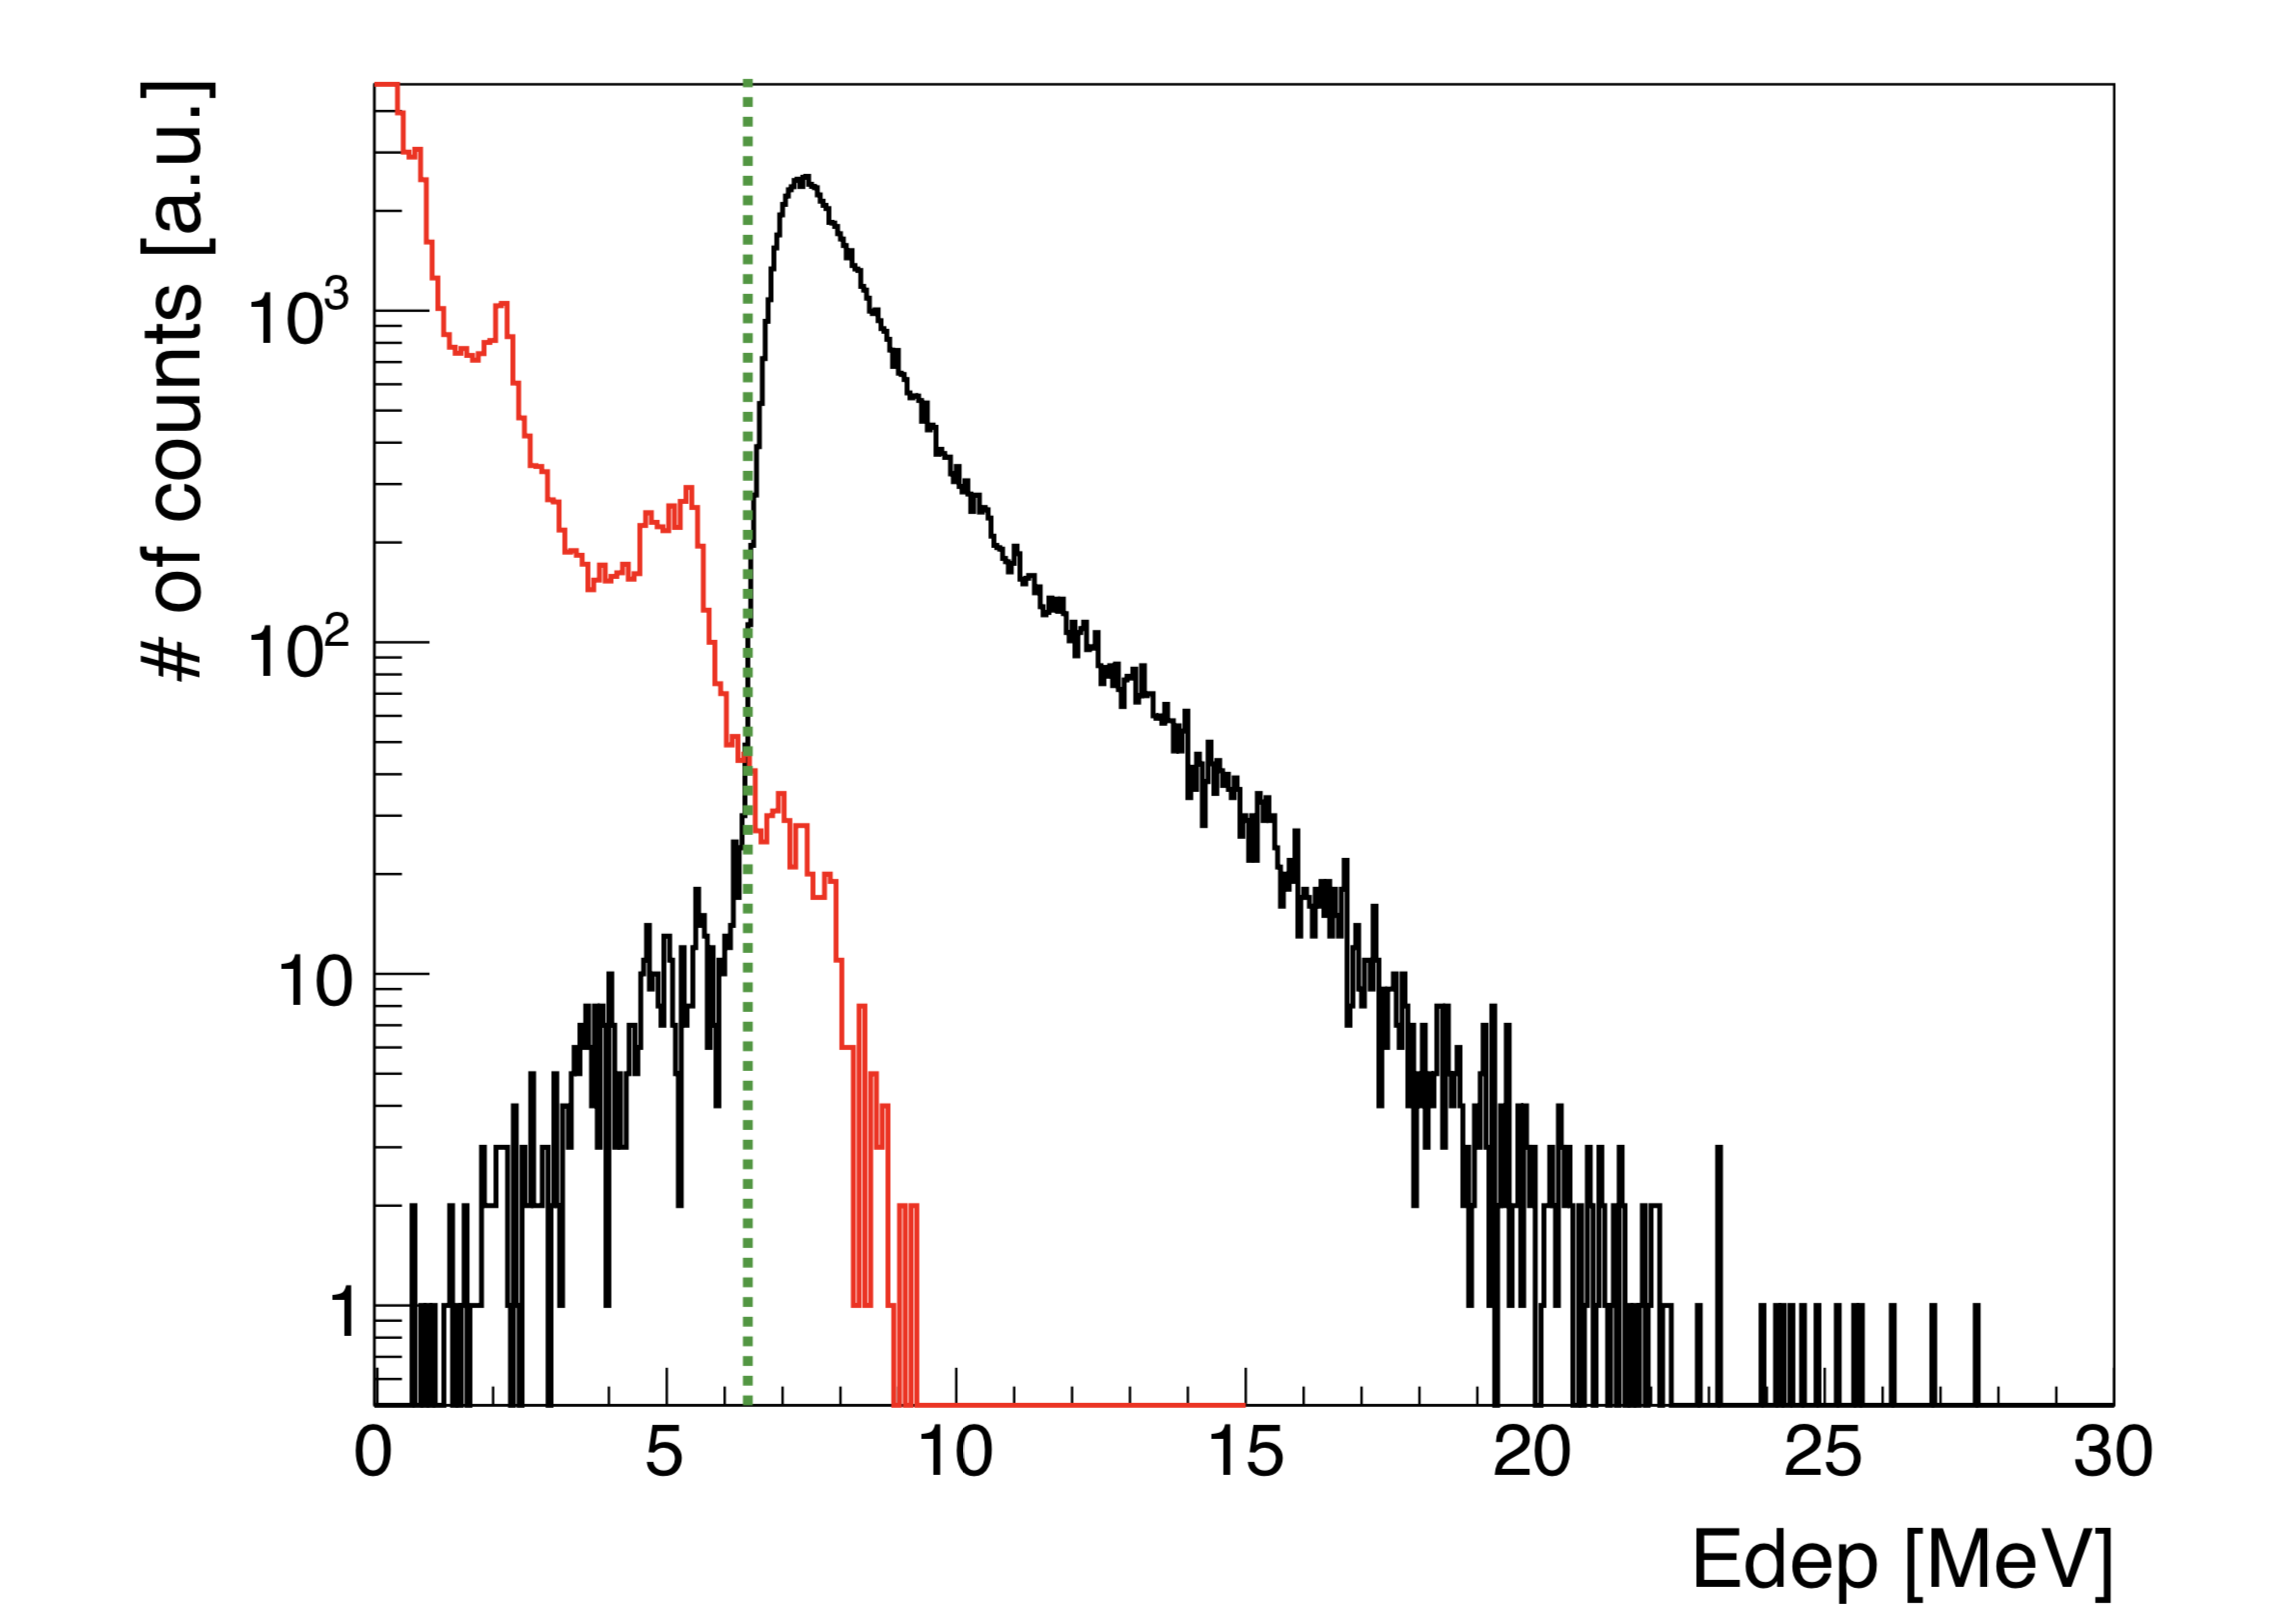
\includegraphics[width=0.7\textwidth]{img/separation}
%\caption{Differences between electrons [black] and X-rays [red] in the energy deposited in the $250$-mm light plastic scintillator. The green dashed line shows a possible location for a cut to separate the particles.}
%\label{fig:separation}
%\end{figure}


\newpage
\section{Interim results}
\paragraph{Planar set-up}
This year various detector configurations have been simulated with the aim of optimising cascade detection efficiency while decreasing the misidentification of electrons as cascade events. One of the geometries is presented in Fig. \ref{fig:setup}.
\begin{figure}[!htbp]
\centering
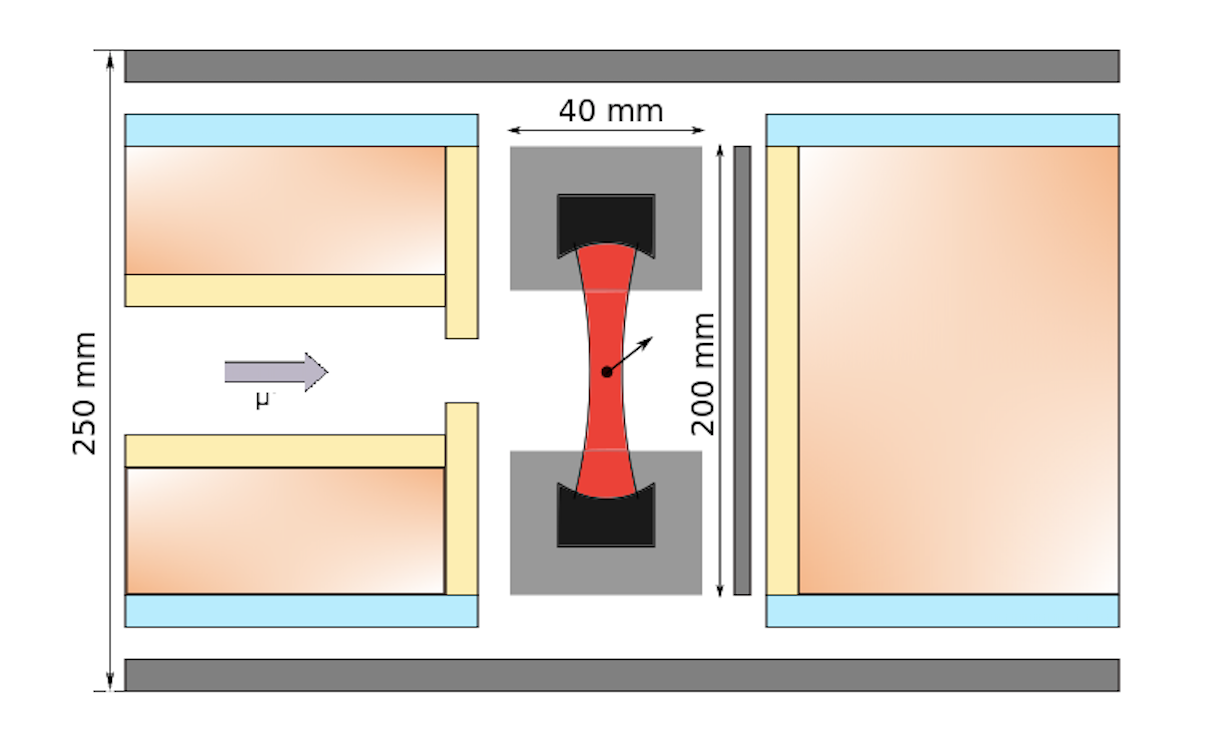
\includegraphics[width=0.8\textwidth]{img/setup4.png}
\caption{Planar detector set-up, with a target and a cavity in the center. Muons are incoming from the left, entering the cavity and getting excited by a laser light. The various thickness scintillating detectors (shown in yellow, orange, and blue) track the energy deposited in them.}
\label{fig:setup}
\end{figure}
In the simulations, the effect of the optical cavity and its mounting mechanics also has to be considered. The major source of electron misidentification arises from $e^-$ impinging on the optical cavity and mounting mechanics that produce bremsstrahlung that is detected in the surrounding plastic scintillators and identified as cascade event (see Fig. \ref{fig:setup}). From this set-up we obtained a cascade event detection probability of $\approx 6.7 \times 10^{-1}$ when the energy cut in the thin scintillator is chosen to bet $0.6$ MeV as can be seen in Fig. \ref{fig:planar_final}.
\begin{figure}[!htbp]
\begin{subfigure}{.485\textwidth}
	\centering
	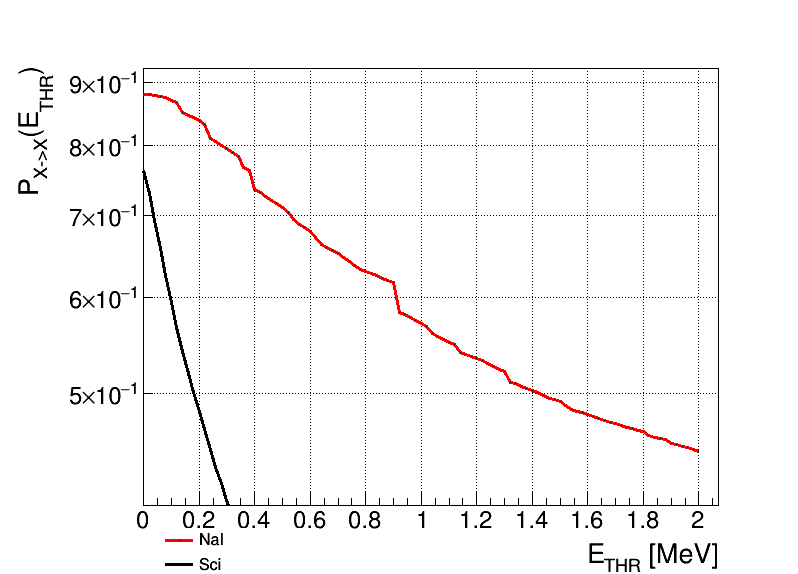
\includegraphics[width=0.97\textwidth]{img/researchplan_planar_final_pxx.png}
	\subcaption{X-ray detection efficiency $P_{X \rightarrow X}$ versus a varying lower energy cut $E_{THR}$.}
	\label{fig:pxx}
\end{subfigure}\hspace*{4.5mm}
\begin{subfigure}{.485\textwidth}
	\centering
	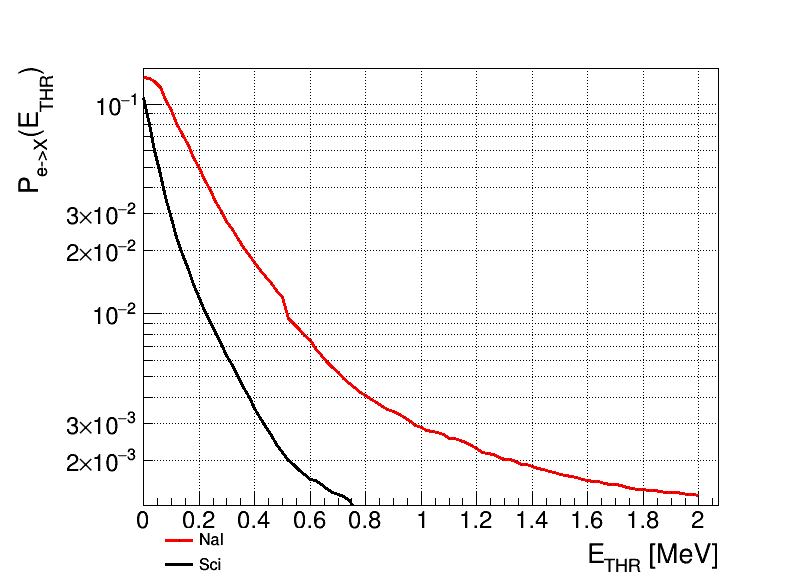
\includegraphics[width=0.97\textwidth]{img/researchplan_planar_final_pex.png}
	\subcaption{Probability that an electron is misidentified as a cascade $P_{e \rightarrow X}$ versus a lower energy cut $E_{THR}$.}
	\label{fig:pex}
\end{subfigure}	
\caption{X-ray detection efficiency $P_{X \rightarrow X}$ and electron misidentification as a cascade probability $P_{e \rightarrow X}$ versus the variable lower energy cut $E_{THR}$ as obtained from the set-up shown in the Fig. \ref{fig:planar_final}. Red and black curves show how the results differ if we use sodium iodide or light plastic scintillation detectors, respectively.}
\label{fig:planar_final}
\end{figure}

\begin{figure}[!htbp]
\begin{subfigure}{.485\textwidth}
	\centering
	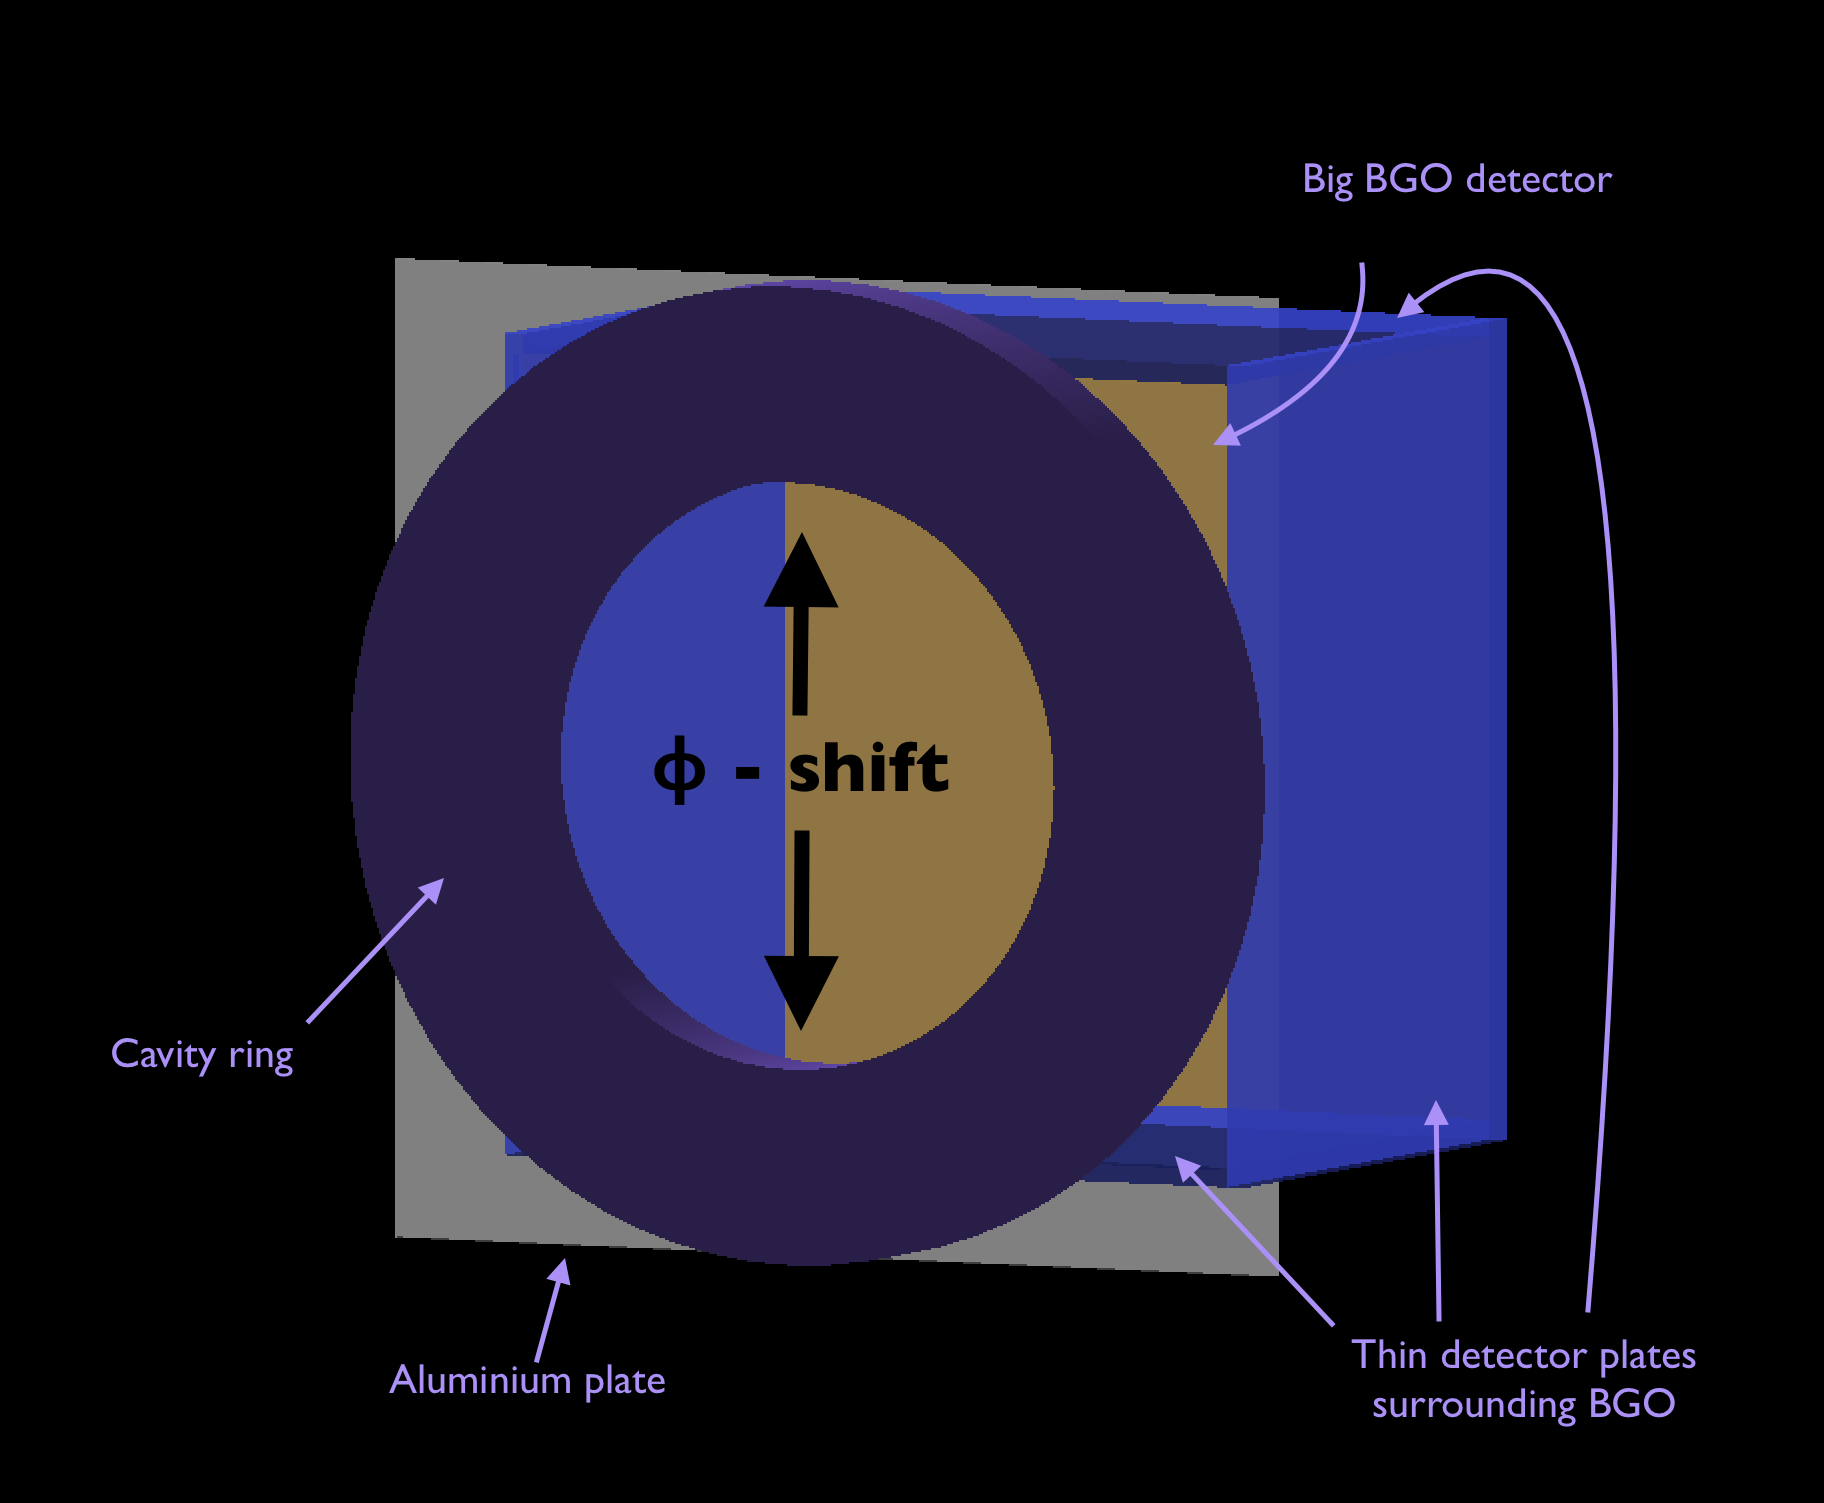
\includegraphics[width=0.97\textwidth]{img/phi-shift.png}
	\subcaption{$\Phi$-shift: changing the inner and outer diameters of the cavity mechanics (shown as a purple ring). A thin aluminium plate is placed behind the cavity representing a target wall. It is followed by a big BGO detector that is surrounded with plates of light plastic scintillation detectors from both sides, top, and the bottom.}
	\label{fig:phishift}
\end{subfigure}\hspace*{4.5mm}
\begin{subfigure}{.485\textwidth}
	\centering
	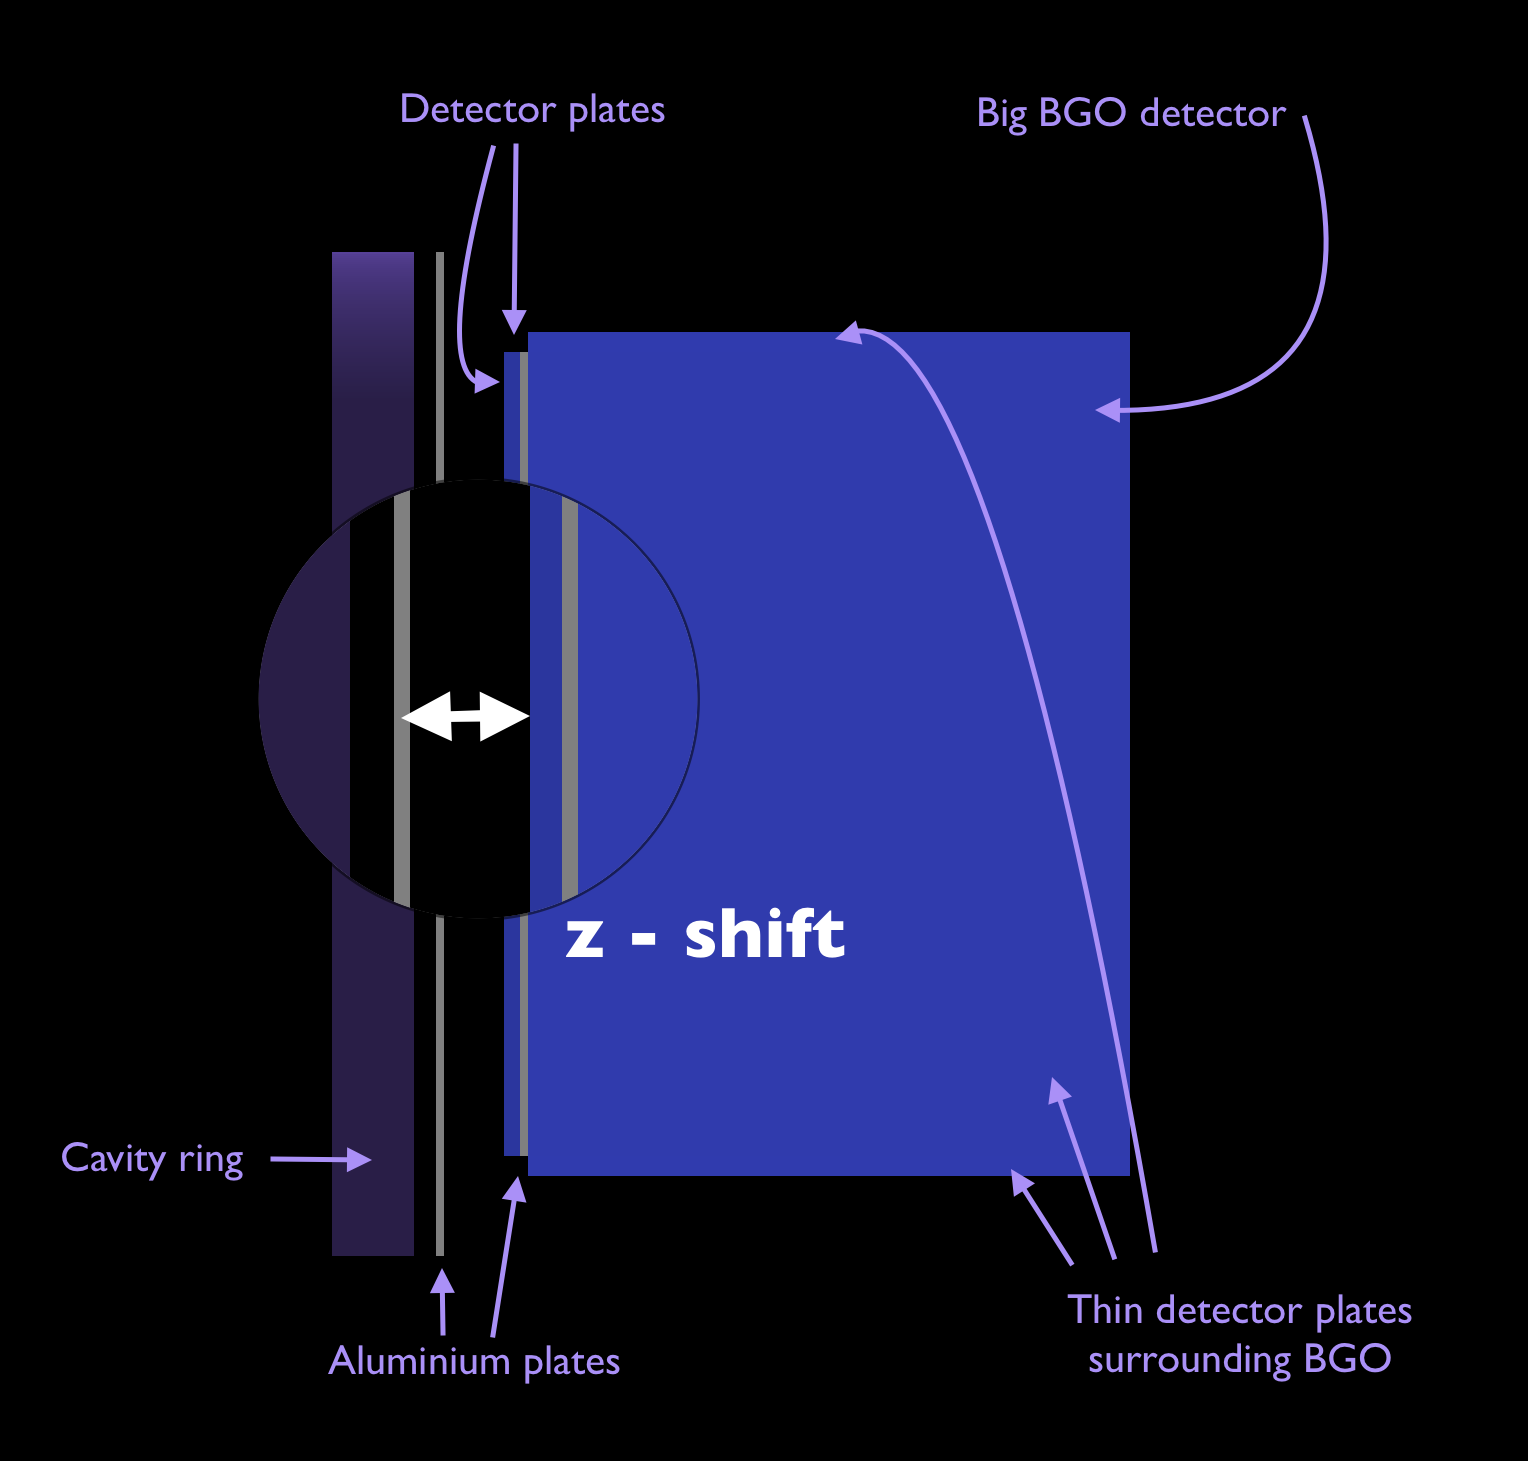
\includegraphics[width=0.835\textwidth]{img/z-shift.png}
	\subcaption{$z$-shift: moving the detectors away from the target. A lateral view to the planar-geometry detection scheme shows two aluminium plates with two thin light plastic scintillation detectors in between them. The big BGO scintillation detector and it surrounding light plastic scintillation detectors are shown on the right.}
	\label{fig:zshift}
\end{subfigure}	
\caption{Optimisation of the $\phi$- and $z$-shifts for the down-stream part of the detector with a planar geometry.}
\label{fig:planarsetup}
\end{figure}


\paragraph{Optimisation of the $\phi$- and $z$-shifts}
In another set-up, where only the down-stream half of the detection system was simulated, the parameters were being optimised by varying the distance between the target cavity with the surrounding mechanics and the detectors. This variation was called the $z$-shift. At the same time, the inner radius of the cavity was also varied introducing the so-called $\phi$-shift (see Fig. \ref{fig:planarsetup}). It was found out that an optical cavity with a diameter of $\phi = 50$-mm and a $z$-shift $z = 0$-mm produce a background at the level of $1 \times 10^{-2}$ applying the $0.5$ MeV lower energy cut. Therefore, an optical cavity of copper is strongly disfavoured. Fig. \ref{fig:misid} shows the cascade event efficiency and electron misidentification as a X-ray probability for various $\phi$- and $z$-shifts.
\begin{figure}[!htbp]
\centering
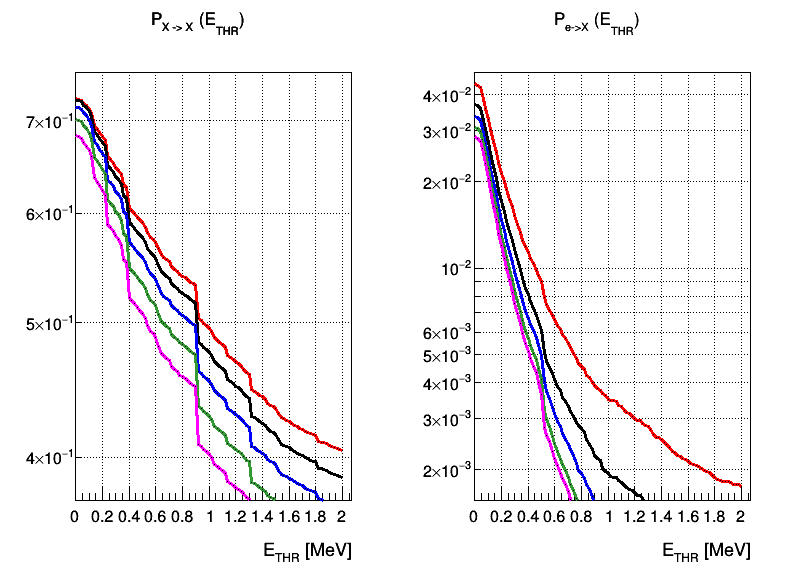
\includegraphics[width=0.86\textwidth]{img/phi_z_shifts.png}
\caption{The variance in the X-ray detection efficiency $P_{X{\rightarrow}X}$ and in the electron misidentification as a X-ray probability $P_{e \rightarrow X}$ for a down-stream planar setup, plotted versus a lower energy threshold $E_{THR}$. Different curves are obtained introducing a fixed $50$-mm $\phi$-shift and \textcolor{red}{$0$-mm}, \textcolor{black}{$25$-mm}, \textcolor{blue}{$50$-mm}, \textcolor{forestgreen(web)}{$75$-mm}, and \textcolor{magenta}{$100$-mm} $z$-shift.}
\label{fig:misid}
\end{figure}

\begin{figure}[!htbp]
\centering
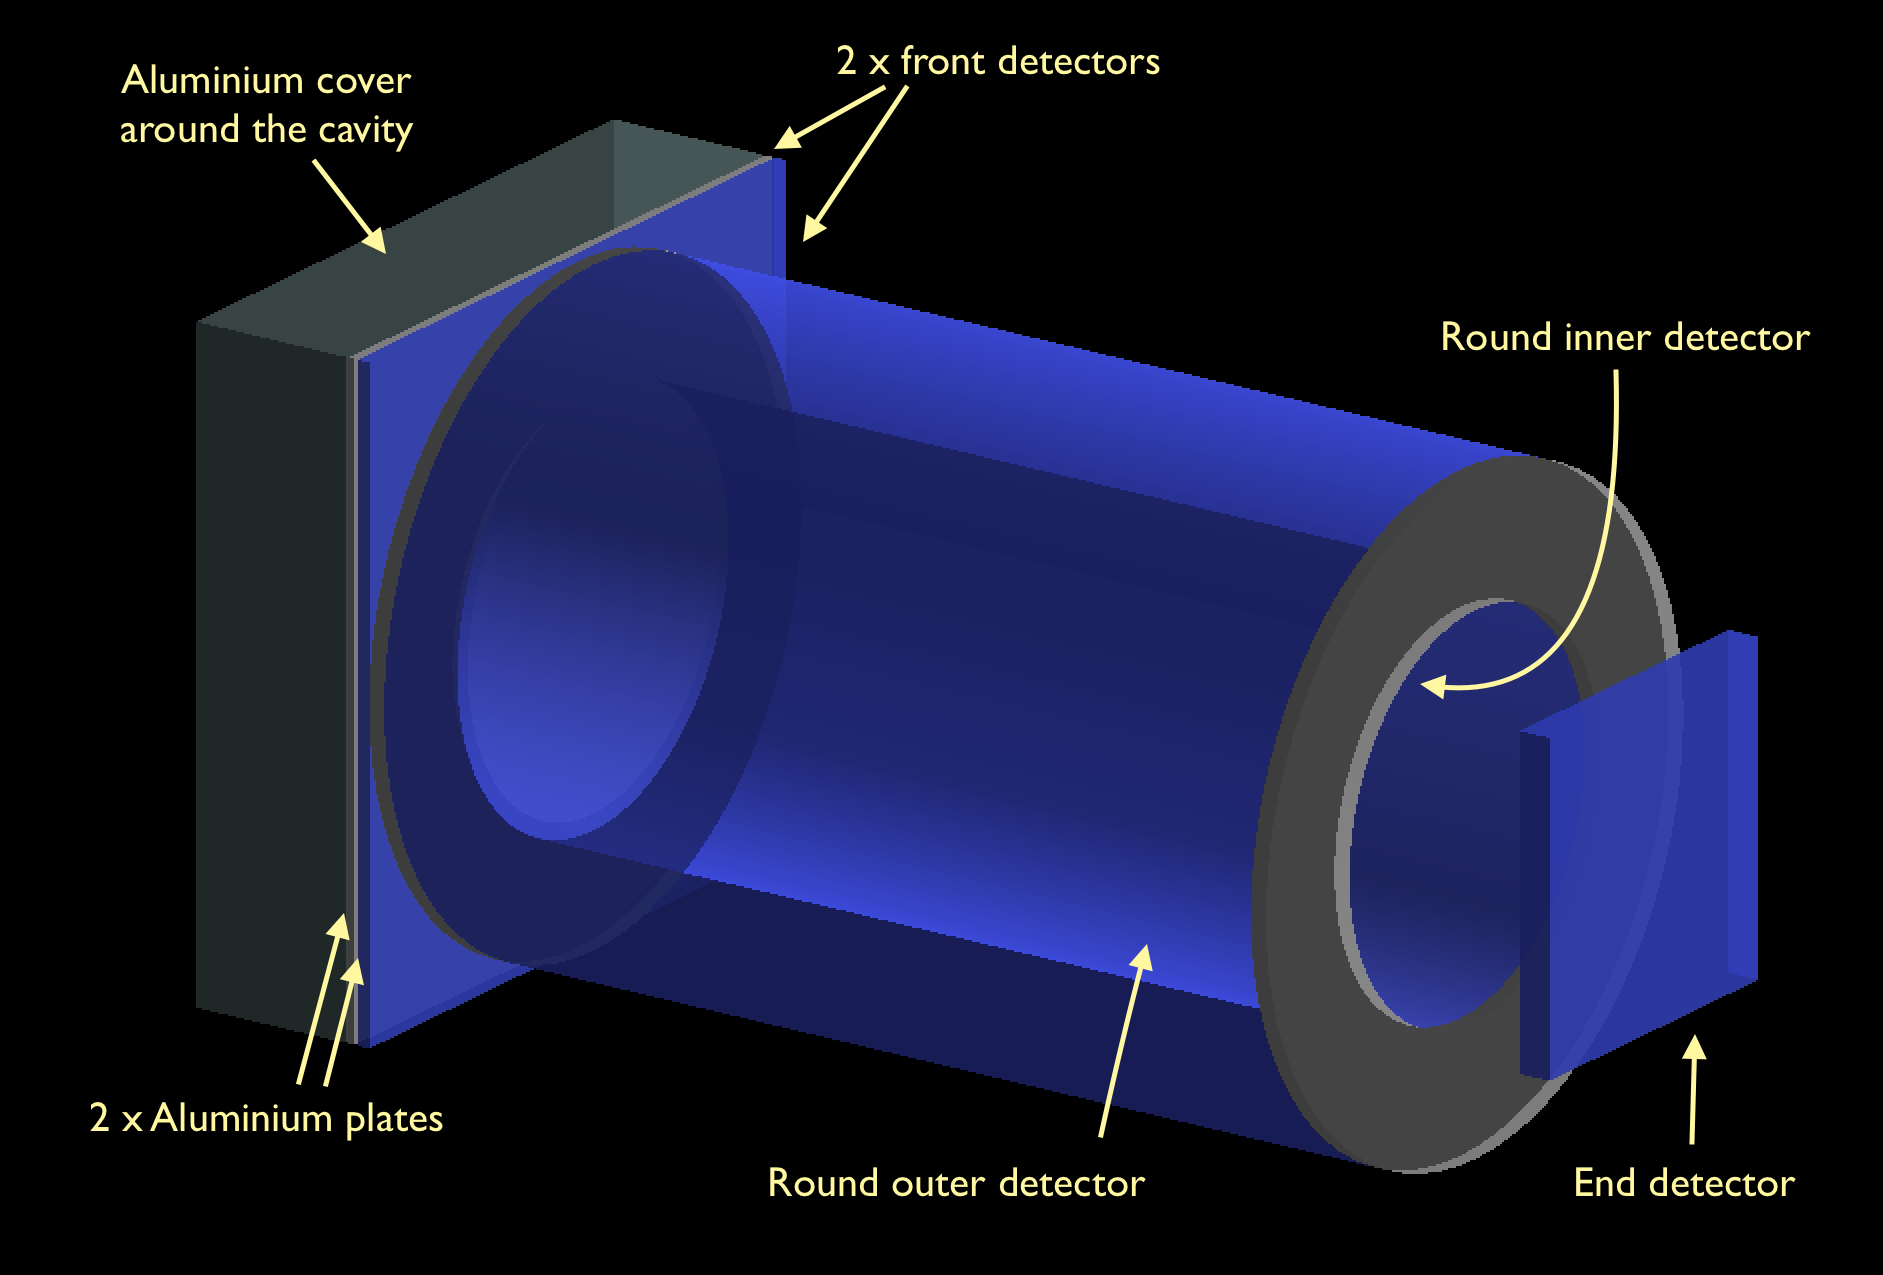
\includegraphics[width=0.6\textwidth]{img/magnetic.png}
\caption{Magnetic setup: a hollow cylindrical scintillation detector in a constant $5$ T magnetic field. Aluminium cover imitates a target area, where $\mu{p}$ atoms are produced. The inner light plastic scintillation detector is topped up with an outer heavier-$Z$ plastic scintillator or, instead, with a layer of aluminium. Between the target and the cylindrical detector there two thin scintillators surrounded by two aluminium plates. At the end of the cylinder [\textit{on the right}] is yet another light plastic scintillator to detect the spiralling electrons exiting the setup.}
\label{fig:magnetic}
%\end{figure}
%\begin{figure}[!htbp]
\centering
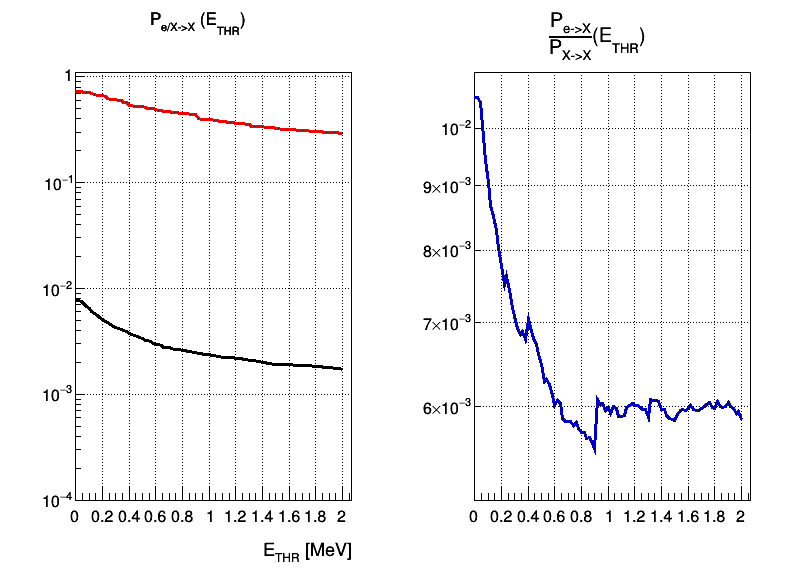
\includegraphics[width=0.8\textwidth]{img/bfield2.png}
\caption{The $e^-$ misidentification probability $P_{e{\rightarrow}X}$ [\textit{black}] and the X-ray detection efficiency $P_{X{\rightarrow}X}$ [\textit{red}] as obtained for the scenario with a magnetic setup.}
\label{fig:bfield}
\end{figure}

\paragraph{Cylindrical detector in a magnetic field}
Another possibility of performing the experiment in a magnetic field was also studied. A hollow scintillating detector with a cylindrical geometry (Fig. \ref{fig:magnetic}) could be used so that $e^-$ do not reach the detector. However, forcing the $e^-$ to spiral into the magnetic field gives rise to an enhanced bremsstrahlung radiation when the $e^-$ crosses the target walls. The left plot in the Fig. \ref{fig:bfield} shows the X-ray detection efficiency $P_{X \rightarrow X}$ [red] and electron misidentification probability $P_{e \rightarrow X}$ [black], whereas their relative ratio $\frac{P_{e \rightarrow X}}{P_{X \rightarrow X}}$ is shown on the right plot in blue. 














%\newpage
\section{Schedule of the research work}
\begin{itemize}
\item[]
%\textbf{\textcolor{forestgreen(web)}{2017 (done)}}
\textbf{1st year [2017 - 2018] (done)}
\begin{itemize}
\item[•]
	Initial detection simulations
\item[•]
	Observation of the development of the single-frequency external cavity tapered amplifier laser system by the researchers from the National Tsing Hua University in Taiwan. 	
\item[•]
	Further detection simulations:
	\begin{itemize}
		\item[$\circ$]
		Geometry, detector materials.
		\item[$\circ$]
		Event - by - event analysis.	
	\end{itemize}
\end{itemize}
%\textbf{\textcolor{harvardcrimson}{2018 (partially done)}}
\item[]
\textbf{2nd year [2018 - 2019]}
\begin{itemize}
\item[•]	
    Advanced detection simulations:
    \begin{itemize}
    		\item[$\circ$]
    		Implementation of the advanced physical processes: nuclear capture and muon transfer, various cascade models.
    \end{itemize}
\item[•]
    Writing of a technical summary of the detector simulations. 
\item[•]
	Simulation of an alternative beam-line in $\pi{e}5$ (if time permits).	 
\item[•]
    Measurements:
    \begin{itemize}
    \item[$\circ$]
	Test of the detection system.
	\item[$\circ$]
    Measure the mean background, mean anti-coincidence detection efficiency.
	\item[$\circ$]
	Measure stopping efficiencies.
	\end{itemize}
\item[•]
	Initial work on Optical Parametric Oscillator (OPO), Optical Parametric Amplifier (OPA), and Difference-Frequency Generator (DFG):
	\begin{itemize}
		\item[$\circ$]
		Check the various schemes and various crystal materials.
		\item[$\circ$]
		Simulation of the scheme and its optimisation.
		\item[$\circ$]
		Test of the scheme in the laboratory.
	\end{itemize}
\end{itemize}
\item[]
\textbf{3rd year [2019 - 2020]}
\begin{itemize}
	\item[•]
	Further work on OPO, OPA, and DFG:
	\begin{itemize}			 
		\item[$\circ$]
		Characterisation of the pulse output.
		\item[$\circ$]
		Spectroscopy of the absorption lines. 
	\end{itemize}		
	\item[•]
    Contribution to the total setup:
	\begin{itemize}
		\item[$\circ$]
		Development and installation of the data acquisition (DAQ) system. 
		\item[$\circ$]
		Target finalisation and installation. 
		\item[$\circ$]
		Detector finalisation and installation.
		\item[$\circ$]
		Laser system's finalisation and installation. 
	\end{itemize}
	\item[•]
	Beam-time, Physics run.
	\item[•]
	Analysis of the beam-time data.
	\item[•]
	Writing of the thesis.
\end{itemize}
%\item[]
%\textbf{4th year [2020 - 2021] (if needed)}
%\begin{itemize}
%	\item[•]
%	Writing of the thesis. 
%\end{itemize}
\end{itemize}
\vspace{3.9pt}


%\newpage
\section{Teaching activities}
\paragraph{}
Previous teaching duties were:
\begin{itemize}
\item
2018 - Teaching assistant for General Physics 2 (FS, Prof. K. Kirch)
\item
2018 - Proton Irradiation Facility (PIF) shift operator (HS, Dr. W. Hajdas)
\end{itemize}
\paragraph{}
Further activities are planned at the PIF at PSI and should occupy $10-13 \%$ of the total workload.\\ 
\vspace{5.1pt}



%\newpage
%\section*{Literature}
\begin{thebibliography}{9}
\bibitem{spectroscopy}
The CREMA collaboration. \textit{Laser Spectroscopy of Muonic Atoms and Ions}. arXiv: 1609.03440v1, 2016.

\bibitem{lambshift}
Aldo Antognini, Franz Kottmann, Fran\c{c}ois Biraben, Paul Indelicato, Fran\c{c}ois Nez, and Randolf Pohl. \textit{Theory of the $2S-2P$ Lamb shift and $2S$ hyperfine splitting in muonic hydrogen}. arXiv: 1208.2637v2, 2012.

\bibitem{proposal}
The CREMA collaboration. \textit{Proposal for an experiment at PSI: Hyperfine splittings in muonic hydrogen and 3He}. 2016.

\bibitem{martynenko}
R. N. Faustov and A. P. Martynenko. \textit{Muonic hydrogen ground state hyperine splitting}. arXiv: hep-ph/0312116v2, 2004.

\bibitem{franziska}
Franziska Hagelstein. \textit{PhD thesis: Exciting nucleons in Compton scattering and hydrogen-like atoms}. arXiv: 1710.00874v1, 2017.

\bibitem{opo}
Xiaobing Xie et al. \textit{Injection-seeded single frequency $2.05$ ${\mu}m$ output by ring cavity optical parametric oscillator}. Chinese Optics Letters, \textbf{15}(9), 2017.

\bibitem{g4beam}
G4beamline software,\\
\url{http://www.muonsinternal.com/muons3/G4beamline}.



%\bibitem{latexcompanion} 
%Michel Goossens, Frank Mittelbach, and Alexander Samarin. 
%\textit{The \LaTeX\ Companion}. 
%Addison-Wesley, Reading, Massachusetts, 1993.
 
%\bibitem{einstein} 
%Albert Einstein. 
%\textit{Zur Elektrodynamik bewegter K{\"o}rper}. (German) 
%[\textit{On the electrodynamics of moving bodies}]. 
%Annalen der Physik, 322(10):891–921, 1905.
 
%\bibitem{knuthwebsite} 
%Knuth: Computers and Typesetting,
%\\\texttt{http://www-cs-faculty.stanford.edu/\~{}uno/abcde.html}
\end{thebibliography}







\end{document}




















